% !TeX program = xelatex
\documentclass[12pt,a4paper]{article}
\usepackage{iftex,mathptmx}
\ifPDFTeX
  \usepackage[utf8]{inputenc}
  \usepackage[T5]{fontenc}
\else
  \usepackage{fontspec}
  \setmainfont{texgyretermes}[Extension=.otf,UprightFont=*-regular,BoldFont=*-bold,ItalicFont=*-italic,BoldItalicFont=*-bolditalic]
  \setmonofont{lmmono10-regular.otf}
\fi
\usepackage[vietnamese]{babel}
\usepackage{amsmath,amssymb,graphicx,booktabs,longtable,tabularx,array,float}
\usepackage[paperwidth=21cm,paperheight=29.7cm,left=3cm,right=2cm,top=2cm,bottom=2.5cm]{geometry}
\usepackage{tikz}
\usetikzlibrary{arrows.meta,positioning,calc}
\usepackage{titlesec,fancyhdr,caption,enumitem,pdflscape,placeins}
\usepackage[unicode]{hyperref}
\hypersetup{colorlinks=true,linkcolor=black,urlcolor=blue,pdftitle={Specification - Bo giai ma Viterbi K=3},pdfauthor={Nhom VLSI}}
\setlength{\parindent}{0.8cm}
\setlength{\parskip}{5pt}
\renewcommand{\baselinestretch}{1.12}
\setlength{\emergencystretch}{2em}
\setlength{\tabcolsep}{5pt}
\renewcommand{\arraystretch}{1.16}
\newcolumntype{Y}{>{\raggedright\arraybackslash}X}
\newcolumntype{P}[1]{>{\raggedright\arraybackslash}p{#1}}
\titleformat{\section}{\centering\bfseries\fontsize{16}{19}\selectfont}{\thesection.}{.5em}{}
\titleformat{\subsection}{\bfseries\fontsize{14}{17}\selectfont}{\thesubsection}{.6em}{}
\titleformat{\subsubsection}{\bfseries\fontsize{12}{15}\selectfont}{\thesubsubsection}{.6em}{}
\titlespacing*{\section}{0pt}{16pt}{10pt}
\titlespacing*{\subsection}{0pt}{12pt}{6pt}
\renewcommand{\figurename}{Hình}
\renewcommand{\tablename}{Bảng}
\captionsetup{font=small,labelfont=bf,skip=7pt}
\pagestyle{fancy}\fancyhf{}
\fancyfoot[L]{\small BTL VLSI -- VITERBI DECODER}
\fancyfoot[R]{\thepage}
\renewcommand{\headrulewidth}{0pt}
\DeclareRobustCommand{\code}[1]{\texttt{#1}}
\let\originalunderscore\_
\renewcommand{\_}{\originalunderscore\allowbreak}
\pdfstringdefDisableCommands{\def\code#1{#1}\def\allowbreak{}}
\setlist[itemize]{topsep=3pt,itemsep=2pt,leftmargin=1.7em}
\setcounter{tocdepth}{2}
\addto\captionsvietnamese{%
  \renewcommand{\contentsname}{MỤC LỤC}%
  \renewcommand{\listfigurename}{DANH MỤC HÌNH}%
  \renewcommand{\listtablename}{DANH MỤC BẢNG}%
  \renewcommand{\refname}{TÀI LIỆU THAM KHẢO}%
}
\begin{document}
\hypersetup{pageanchor=false}
\begin{titlepage}
\thispagestyle{empty}
\centering
\setlength{\parskip}{0pt}
\begin{tikzpicture}[remember picture,overlay]
\draw[line width=2pt] ($(current page.north west)+(3cm,-2cm)$) rectangle ($(current page.south east)+(-2cm,2.5cm)$);
\draw[line width=.45pt] ($(current page.north west)+(3.12cm,-2.12cm)$) rectangle ($(current page.south east)+(-2.12cm,2.62cm)$);
\end{tikzpicture}\par
\vspace*{\fill}
{\large\bfseries ĐẠI HỌC BÁCH KHOA HÀ NỘI\\[3pt]
TRƯỜNG ĐIỆN -- ĐIỆN TỬ\par}
\vspace{0.9cm}

\includegraphics[height=3.65cm]{Images/logodhbk.png}\par
\vspace{1.2cm}
{\Huge\bfseries BÁO CÁO BÀI TẬP LỚN\par}
\vspace{0.5cm}
{\large\bfseries HỌC PHẦN: VLSI\par}
\vspace{0.85cm}
{\Large\bfseries ĐẶC TẢ THIẾT KẾ (SPECIFICATION)\\[4pt]
BỘ GIẢI MÃ VITERBI\par}
\vspace{1.0cm}
{\normalsize
\begin{tabular}{@{}l@{\hspace{1.1cm}}l@{}}
\textbf{Sinh viên thực hiện:} & Vũ Thanh Hằng -- 20233385\\[5pt]
                             & Đinh Thị Tuyết Mai -- 20233516\\[5pt]
                             & Lương Ngọc Minh -- 20233529\\[12pt]
\textbf{GV hướng dẫn:}       & TS. Nguyễn Vũ Thắng
\end{tabular}\par}
\vspace*{\fill}
\end{titlepage}
\hypersetup{pageanchor=true}
\pagenumbering{roman}
\tableofcontents\clearpage
\phantomsection
\addcontentsline{toc}{section}{\listfigurename}
\listoffigures\clearpage
\phantomsection
\addcontentsline{toc}{section}{\listtablename}
\listoftables\clearpage
\section*{DANH MỤC CHỮ VIẾT TẮT}
\addcontentsline{toc}{section}{DANH MỤC CHỮ VIẾT TẮT}
\begin{tabularx}{\textwidth}{@{}P{1.8cm}Y@{}}\toprule
BMU & Branch Metric Unit: khối tính độ sai khác của từng nhánh trellis.\\
ACS & Add--Compare--Select: cộng, so sánh và chọn đường sống sót.\\
PM & Path Metric: tổng khoảng cách của đường đi đến một trạng thái.\\
SM & Survivor Memory: bộ nhớ lưu quyết định chọn đường.\\
TB & Traceback: truy vết ngược để khôi phục các bit thông tin.\\
FSM & Finite State Machine: máy trạng thái hữu hạn.\\
RTL & Register Transfer Level: mức mô tả thanh ghi và truyền dữ liệu.\\
STA & Static Timing Analysis: phân tích thời gian tĩnh.\\
PPA & Power, Performance, Area: công suất, hiệu năng và diện tích.\\
\bottomrule\end{tabularx}
\clearpage\pagenumbering{arabic}

% BEGIN ALGORITHM STUDY
\clearpage
\section{TÌM HIỂU MÃ CHẬP VÀ THUẬT TOÁN VITERBI}\label{sec:algorithm}

\subsection{Tổng quan bài toán giải mã và mã chập $(7,5)_8$}

\subsubsection{Bài toán khôi phục dữ liệu trên kênh có nhiễu}
Một bộ giải mã sửa lỗi cần giải quyết hai nhiệm vụ: xác định tập những chuỗi hợp lệ có thể được phát và tìm chuỗi phù hợp nhất với quan sát thu được ở đầu thu. Chỉ nhìn vào một bit nhận riêng lẻ thường chưa đủ, vì giá trị 0 hoặc 1 đều có thể là dữ liệu gốc hoặc kết quả của lỗi kênh. Mã hóa kênh đưa thêm quan hệ ràng buộc giữa các bit để đầu thu có căn cứ phân biệt các khả năng đó.

Trong mã chập (convolutional code), quan hệ ràng buộc trải qua nhiều thời điểm liên tiếp. Mỗi nhóm bit mã hóa phụ thuộc cả bit thông tin hiện tại lẫn một số bit trước đó. Vì thế, một quyết định ở hiện tại phải nhất quán với lịch sử của bộ mã hóa (encoder). Một symbol trông rất hợp lý nếu xét riêng có thể làm chuỗi trạng thái mất tính liên tục; ngược lại, chấp nhận một sai khác nhỏ tại symbol hiện tại có thể tạo được đường đi tối ưu hơn cho toàn bộ khung.

\begin{figure}[H]\centering
\begin{tikzpicture}[>=Stealth,box/.style={draw,rounded corners,align=center,minimum height=1.15cm,font=\small}]
\node[box,text width=2.5cm] (a) at (0,0) {Bit thông tin\\$u_0,u_1,\ldots$};
\node[box,text width=2.5cm] (b) at (3.5,0) {Encoder mã chập\\chuỗi hợp lệ $v$};
\node[box,text width=2.1cm] (c) at (6.9,0) {Kênh có nhiễu\\quan sát $r$};
\node[box,text width=2.6cm] (d) at (10.4,0) {Viterbi decoder\\ước lượng $\hat u$};
\draw[->] (a)--(b);\draw[->] (b)--(c);\draw[->] (c)--(d);
\end{tikzpicture}
\caption{Vị trí của Viterbi decoder trong chuỗi truyền tin}\label{fig:theory-chain}
\end{figure}

Với cấu hình $R=1/2$, encoder tạo hai bit mã cho mỗi bit thông tin. Việc tăng số bit truyền tạo ra độ dư để sửa lỗi, nhưng đồng thời làm tăng băng thông hoặc thời gian truyền nếu tốc độ bit trên kênh giữ nguyên. Do đó, lợi ích sửa lỗi luôn cần được đánh giá cùng tốc độ mã, độ trễ, dung lượng bộ nhớ và năng lượng xử lý. Thuật toán Viterbi giải bài toán tìm một \emph{chuỗi} phù hợp nhất trên đồ thị trellis, sau đó ánh xạ trực tiếp từng thao tác sang phần cứng; cơ sở về branch metric, path metric và truy hồi được đối chiếu với bài giảng MIT 6.02, còn phần tổ chức bộ nhớ được tham khảo thêm từ luận văn của O'Shea \cite{mit-lecture,oshea-thesis}.

\subsubsection{Bộ nhớ encoder, chiều dài ràng buộc và đa thức sinh}
Với encoder nhị phân nhận $k=1$ bit vào và xuất $n=2$ bit ra mỗi bước, gọi $m$ là số phần tử nhớ và $K=m+1$ là chiều dài ràng buộc (constraint length). Một đầu ra phụ thuộc tối đa $K$ bit: bit vào hiện tại và $m$ bit lưu trong thanh ghi dịch. Số trạng thái bộ nhớ là $S=2^m=2^{K-1}$. Với cấu hình của dự án, $K=3$ tương ứng chỉ có $m=2$ bit nhớ và $S=4$ trạng thái (bộ ba $(n,k,m)=(2,1,2)$). Cần tránh nhầm lẫn với cấu hình $(2,1,3)$ có ba bit nhớ và tám trạng thái trong luận văn O'Shea \cite[Chương 2]{oshea-thesis}, nên không thể lấy nguyên bảng chuyển trạng thái của tài liệu đó cho bản RTL này.

\begin{figure}[H]\centering
\begin{tikzpicture}[>=Stealth,thick]
\node[draw,minimum width=2cm,minimum height=1cm] (a) at (3,0) {$a=u_{t-1}$};
\node[draw,minimum width=2cm,minimum height=1cm] (b) at (7,0) {$b=u_{t-2}$};
\draw[->] (0,0) node[left]{$u_t$}--(a);\draw[->] (a)--(b);\draw[->] (b)--(9,0);
\node[align=center] at (4.5,-1.3) {Sau một bước: $a^+=u_t$, $b^+=a$\\Trạng thái hiện tại: $s_t=(a,b)$};
\end{tikzpicture}
\caption{Hai phần tử nhớ của encoder có $K=3$}\label{fig:theory-encoder}
\end{figure}

Trạng thái $s_t=(a,b)$ không lưu toàn bộ bản tin đã phát mà chỉ giữ phần lịch sử còn ảnh hưởng đến các đầu ra tương lai. Hai chuỗi quá khứ khác nhau nhưng kết thúc ở cùng $(a,b)$ sẽ có tập chuyển tiếp tương lai hoàn toàn giống nhau. Tính chất này cho phép thuật toán Viterbi gộp nhiều lịch sử thành một đại diện duy nhất tại mỗi trạng thái. Khi tăng $K$, ràng buộc sửa lỗi mạnh hơn nhưng số trạng thái tăng theo hàm mũ $2^{K-1}$ và số nhánh mỗi bước bằng $2S$ (Bảng~\ref{tab:theory-kscale}); encoder chỉ cần thêm vài flip-flop và cổng XOR, trong khi decoder phải theo dõi đồng thời mọi trạng thái, khiến phần cứng giải mã phình to nhanh hơn nhiều so với phần cứng mã hóa.

\begin{table}[H]\centering\small
\begin{tabular}{cccc}\toprule
\textbf{$K$}&\textbf{Bit nhớ $m$}&\textbf{Số state $2^m$}&\textbf{Số nhánh mỗi bước ($2S$)}\\\midrule
3&2&4&8\\4&3&8&16\\5&4&16&32\\7&6&64&128\\\bottomrule
\end{tabular}
\caption{Ảnh hưởng của chiều dài ràng buộc đến kích thước trellis}\label{tab:theory-kscale}
\end{table}

Đa thức sinh mô tả các điểm lấy tín hiệu đưa vào bộ cộng modulo 2 trên trường $\mathrm{GF}(2)$ (phép XOR, $1+1=0$ không nhớ). Với cặp $(7,5)_8$, biểu diễn nhị phân lần lượt là $111$ và $101$, tương ứng:
\begin{equation}
g_0(D)=1+D+D^2,\qquad g_1(D)=1+D^2,
\end{equation}
trong đó $D$ biểu diễn một bước trễ. Hệ số 1 tại $D$ cho biết có nối phần tử nhớ thứ nhất vào cổng XOR, còn hệ số 0 cho biết bỏ qua. Do đó, hai bit đầu ra tại thời điểm $t$ là:
\begin{equation}
v_{0,t}=u_t\oplus u_{t-1}\oplus u_{t-2},\qquad
v_{1,t}=u_t\oplus u_{t-2}.
\end{equation}
Ví dụ, với chuỗi thông tin theo thời gian $1,0,0$ từ trạng thái đầu `00`, các symbol phát lần lượt là `11`, `10`, `11`; bit 1 đầu tiên vẫn ảnh hưởng đến hai lần mã hóa tiếp theo dù các bit vào sau đều bằng 0. Biểu diễn đa thức $V_0(D)=U(D)g_0(D)$ và $V_1(D)=U(D)g_1(D)$ thuận tiện khi phân tích tính chất mã, còn dạng thanh ghi dịch thuận tiện khi thiết kế RTL. Hai công thức trên phải được giữ đúng thứ tự giữa encoder, mô hình tham chiếu và decoder: đổi từ $(7,5)_8$ sang $(5,7)_8$ sẽ đảo vị trí hai bit trong mỗi symbol và đòi hỏi phải đổi tương ứng cả bus nhận lẫn nhãn trellis.

\subsubsection{Quy ước ký hiệu, thứ tự bit và thời gian}
Nhiều sai lệch khi đối chiếu tài liệu không đến từ thuật toán mà từ quy ước đặt tên bit và đóng gói từ nhị phân. Báo cáo thống nhất bộ ký hiệu trong Bảng~\ref{tab:theory-notation}: trong mỗi symbol 2 bit, bit cao biểu diễn $v_0$ và bit thấp biểu diễn $v_1$; mã trạng thái có dạng $\{a,b\}$ với $a$ là bit thông tin mới hơn. Do đó, mã state `10` và symbol mã hóa `10` là hai đối tượng hoàn toàn khác nhau dù cùng rộng 2 bit.

\begin{table}[H]\centering\small
\begin{tabularx}{\textwidth}{@{}P{3cm}Y@{}}\toprule
\textbf{Ký hiệu}&\textbf{Nội dung}\\\midrule
$t=0,\ldots,L-1$&Chỉ số symbol theo thời gian, không phải chỉ số cạnh clock của FSM.\\
$s_t=(a,b)$&Trạng thái trước bước $t$; $s_0=00$ khi biết trạng thái đầu.\\
$s_{t+1}=(u_t,a)$&Trạng thái đích sau bước $t$.\\
$PM_t(s)$&Path metric tối ưu sau khi đã xử lý đúng $t$ symbol.\\
$M[t][j]$&Bit quyết định (decision) của state đích $j$ sau khi xử lý $r_t$.\\
$d_{xy}(r_t)$&Khoảng cách Hamming của symbol nhận $r_t$ đến cặp bit $xy$.\\\bottomrule
\end{tabularx}
\caption{Bảng ký hiệu dùng thống nhất cho phần thuật toán}\label{tab:theory-notation}
\end{table}

Ở chế độ mặc định \code{MSB\_FIRST=0}, bit $u_0$ nằm ở \code{decoded\_data[0]} và symbol $r_0$ nằm ở \code{encoded\_data[1:0]}:
\begin{equation}
U_{\mathrm{LSB}}=\sum_{t=0}^{L-1}u_t2^t,\qquad
R_{\mathrm{LSB}}=\sum_{t=0}^{L-1}r_t2^{2t}.
\end{equation}
Vì các số thập lục phân (hex) in bit trọng số cao ở bên trái, không thể đọc chuỗi thời gian trực tiếp từ trái sang phải của một số hex. Chẳng hạn, byte \code{8'h37} có dạng nhị phân `00110111`, nhưng chuỗi thông tin theo thời gian ở chế độ LSB-first là `11101100`. Chế độ \code{MSB\_FIRST=1} đảo ngược vị trí đóng gói các symbol và bit thông tin trên bus mà không làm thay đổi quan hệ chuyển trạng thái.

\subsection{Biểu diễn trạng thái và đồ thị Trellis}
Encoder có bộ nhớ hữu hạn là một máy trạng thái: cặp $(s_t, u_t)$ quyết định duy nhất cả symbol phát $v_0v_1$ lẫn trạng thái kế tiếp $s_{t+1}$. Với hai bit nhớ, tám tổ hợp tạo thành tám nhánh chuyển có hướng (Bảng~\ref{tab:theory-trellis}). Nhìn theo chiều đi, state `10` chuyển sang `01` hoặc `11`; nhìn theo chiều đến, state `01` chỉ nhận nhánh từ `10` hoặc `11`. Encoder sử dụng chiều đi để phát symbol, còn decoder sử dụng chiều đến để so sánh các nhánh hội tụ vào từng state đích.

\begin{table}[H]\centering\small
\begin{tabular}{cccc}\toprule
\textbf{Trạng thái trước $s_t$}&\textbf{Bit vào $u_t$}&\textbf{Trạng thái kế $s_{t+1}$}&\textbf{Nhãn nhánh $u/v_0v_1$}\\\midrule
00&0&00&0/00\\00&1&10&1/11\\01&0&00&0/11\\01&1&10&1/00\\
10&0&01&0/10\\10&1&11&1/01\\11&0&01&0/01\\11&1&11&1/10\\\bottomrule
\end{tabular}
\caption{Bảng chuyển trạng thái tám nhánh của encoder $(7,5)_8$}\label{tab:theory-trellis}
\end{table}

Một hệ quả rất thuận lợi cho phần cứng là bit cao của trạng thái đích bằng chính bit thông tin $u$ vừa đi vào (nếu state đích là `01` thì chắc chắn $u=0$; nếu là `10` thì $u=1$). Tuy nhiên, state đích chưa xác định duy nhất trạng thái trước (predecessor) vì còn thiếu bit nhớ cũ của state trước:
\begin{equation}
j=(u,a)\quad\Longrightarrow\quad
p_0=(a,0),\quad p_1=(a,1).
\end{equation}
Do đó, một bit decision duy nhất do khối ACS chọn là đủ để phân biệt hai predecessor đi vào mỗi state đích. Nếu thay đổi quy ước sắp xếp bit trong state thì công thức predecessor và toàn bộ logic truy vết cũng phải đổi tương ứng.

Vì sơ đồ trạng thái không có trục thời gian nên các nhánh tạo thành vòng lặp. Khi trải sơ đồ theo từng thời điểm cho chuỗi dài $L$ symbol, ta thu được đồ thị trellis gồm $L+1$ cột trạng thái đi từ trái sang phải (Hình~\ref{fig:theory-trellis}). Mỗi đường liên tục từ cột $s_0$ đến cột $s_L$ tương ứng với một chuỗi thông tin hợp lệ.

\begin{figure}[H]\centering
\begin{tikzpicture}[x=2.45cm,y=1.25cm,>=Stealth,font=\small]
\foreach \t in {0,1,2,3,4}{\foreach \s/\lab in {0/00,1/01,2/10,3/11}{\node[circle,fill,inner sep=1.8pt] (n\t\s) at (\t,-\s) {};\ifnum\t=0\node[left] at (n\t\s) {\lab};\fi}\node at (\t,.5) {$s_{\t}$};}
\foreach \t/\n in {0/1,1/2,2/3,3/4}{
\foreach \p/\d in {0/0,1/0,2/1,3/1}{\draw[->,gray] (n\t\p)--(n\n\d);}
\foreach \p/\d in {0/2,1/2,2/3,3/3}{\draw[->,gray,dashed] (n\t\p)--(n\n\d);}}
\draw[->,very thick] (n00)--(n12);\draw[->,very thick] (n12)--(n21);\draw[->,very thick] (n21)--(n30);\draw[->,very thick] (n30)--(n42);
\node[align=center] at (2,-4) {Nét liền: $u=0$; nét đứt: $u=1$\\Đường đậm: chuỗi $1,0,0,1$ từ state 00};
\end{tikzpicture}
\caption{Trellis bốn bước theo quy ước state của báo cáo}\label{fig:theory-trellis}
\end{figure}

Khi biết $s_0=00$, sau bước đầu tiên chỉ có hai state `00` và `10` có thể tới; từ bước thứ hai trở đi cả bốn state đều có đường hợp lệ. Dù hình vẽ thể hiện đủ mọi cạnh, decoder phải biểu diễn các nút chưa thể tới ở hai bước đầu bằng metric vô cực. Ngoài ra, trellis làm rõ quan hệ đánh chỉ số bộ nhớ: hàng survivor tại địa chỉ $t$ lưu quyết định của các nhánh đi tới cột $t+1$, nên khi truy vết từ $s_{t+1}$ phải đọc hàng $t$ (không phải hàng $t+1$) để tránh làm lệch toàn bộ chuỗi bit đầu ra.

\subsection{Cơ sở thuật toán Viterbi}

\subsubsection{Hạn chế của chọn nhánh cục bộ và tiêu chuẩn Maximum Likelihood}
Nếu ở mỗi bước ta chọn ngay nhánh có khoảng cách Hamming nhỏ nhất (tham lam theo từng symbol) và chỉ giữ một đường duy nhất, một lỗi kênh có thể kéo bộ giải mã sang trạng thái sai. Chẳng hạn, xét hai đường kết thúc ở hai trạng thái khác nhau với metric lần lượt là 1 và 2; nếu ở bước kế tiếp đường thứ nhất tăng thêm 2 còn đường thứ hai khớp hoàn toàn (tăng 0), tổng metric trở thành 3 và 2 — đường thứ hai mới là đường tốt hơn. Vì vậy, chưa thể loại một đường chỉ vì metric tạm thời lớn hơn khi chúng đang ở hai trạng thái khác nhau. Ngược lại, tìm kiếm vét cạn trên cả $2^L$ chuỗi thông tin tuy tối ưu nhưng không khả thi khi $L$ tăng (ví dụ $L=100$ có $2^{100}$ chuỗi). Thuật toán Viterbi kết hợp ưu điểm của cả hai bằng cách giữ đúng một đường tốt nhất cho \emph{mỗi trạng thái} tại mỗi thời điểm (Bảng~\ref{tab:theory-compare}), đưa độ phức tạp về tuyến tính theo chiều dài khung $L$.

\begin{table}[H]\centering\small
\begin{tabularx}{\textwidth}{@{}P{3.1cm}P{3.2cm}Y@{}}\toprule
\textbf{Phương pháp}&\textbf{Thông tin lưu lại}&\textbf{Đặc điểm}\\\midrule
Chọn nhánh từng bước&Một đường nhỏ nhất tại bước đang xét&Có thể loại mất đường tối ưu khi xét cả chuỗi.\\
Tìm kiếm vét cạn&Toàn bộ $2^L$ chuỗi thông tin&Tìm được nghiệm tối ưu, nhưng độ phức tạp tăng theo hàm mũ $2^L$.\\
Viterbi&Một đường tốt nhất cho mỗi state&Loại các đường kém hơn khi cùng hội tụ tại một state; độ phức tạp tuyến tính theo $L$.\\\bottomrule
\end{tabularx}
\caption{So sánh chọn nhánh từng bước, tìm kiếm vét cạn và Viterbi}\label{tab:theory-compare}
\end{table}

Giải mã theo tiêu chuẩn Maximum Likelihood (ML) là chọn từ mã hợp lệ $v$ cực đại hóa xác suất điều kiện $P(r\mid v)$. Xét kênh đối xứng nhị phân (BSC) với xác suất lật bit $p$ ($0<p<1/2$) và lỗi ở các bit độc lập nhau. Với các từ mã cùng độ dài $N_c$ bit, nếu $r$ khác $v$ ở $d$ vị trí thì:
\begin{equation}
P(r\mid v)=p^d(1-p)^{N_c-d},
\end{equation}
\begin{equation}
-\log P(r\mid v)=-N_c\log(1-p)+d\log\frac{1-p}{p}.
\end{equation}
Do $N_c$ và $p$ không đổi trên cả khung và $\log\frac{1-p}{p}>0$ khi $p<1/2$, tối đa hóa $P(r\mid v)$ tương đương với tối thiểu hóa khoảng cách Hamming $d$ giữa $r$ và $v$ \cite[Mục 9.2]{mit-lecture}. Bảng~\ref{tab:theory-bsc} tóm tắt các giả thiết đứng sau sự tương đương này. Lưu ý rằng Viterbi tối ưu xác suất đúng của \emph{cả chuỗi} (ML sequence), khác với các phương pháp như MAP/BCJR vốn tối ưu xác suất lỗi trên từng bit riêng lẻ.

\begin{table}[H]\centering\small
\begin{tabularx}{\textwidth}{@{}P{4cm}Y@{}}\toprule
\textbf{Giả thiết}&\textbf{Ý nghĩa khi tính metric}\\\midrule
Lỗi ở các bit độc lập&Xác suất chuỗi viết thành tích; khi lấy logarit trở thành tổng cộng dồn.\\
Xác suất lật bit như nhau&Mỗi vị trí sai khác đóng góp cùng một trọng số vào metric.\\
$p<1/2$&Từ mã có ít vị trí sai khác hơn luôn có xác suất hợp lý lớn hơn.\\
Các từ mã cùng độ dài&Số hạng phụ thuộc $N_c$ giống nhau nên không ảnh hưởng thứ tự so sánh.\\\bottomrule
\end{tabularx}
\caption{Các giả thiết khi dùng khoảng cách Hamming làm metric ML}\label{tab:theory-bsc}
\end{table}

\subsubsection{Branch Metric, Path Metric và thao tác Add--Compare--Select}
Branch metric là chi phí gắn với một cạnh trellis tại thời điểm $t$. Với quan sát cứng $r_t=(r_1,r_0)$ và symbol dự kiến $v=(v_1',v_0')$, chi phí là tổng số học hai bit sai khác:
\begin{equation}
BM_t(v)=(r_1\oplus v_1')+(r_0\oplus v_0')\in\{0,1,2\}.
\end{equation}
Không thể thay dấu cộng số học bằng một phép XOR duy nhất giữa hai bit sai khác vì trường hợp sai cả hai bit sẽ cho kết quả 0. Do tám cạnh trellis chỉ sử dụng bốn nhãn đầu ra $\{00,01,10,11\}$, khối BMU chỉ cần tính bốn khoảng cách dùng chung một lần (Bảng~\ref{tab:theory-bm4}) rồi phân phối tới bốn khối ACS; quan hệ giữa nhãn nhánh và state đích nằm ở sơ đồ nối dây của ACS unit.

\begin{table}[H]\centering\small
\begin{tabular}{ccccc}\toprule
\textbf{Symbol nhận}&\textbf{Tới 00}&\textbf{Tới 01}&\textbf{Tới 10}&\textbf{Tới 11}\\\midrule
00&0&1&1&2\\01&1&0&2&1\\10&1&2&0&1\\11&2&1&1&0\\\bottomrule
\end{tabular}
\caption{Bốn khoảng cách Hamming dùng chung cho mọi nhánh trellis}\label{tab:theory-bm4}
\end{table}

Gọi $\mathcal P_t(j)$ là tập các đường hợp lệ từ trạng thái đầu tới state $j$ sau $t$ symbol. Path metric tối ưu tại nút đó được định nghĩa là:
\begin{equation}
PM_t(j)=\min_{P\in\mathcal P_t(j)}\sum_{\tau=0}^{t-1}BM_\tau(P),
\end{equation}
và bằng $\infty$ nếu $\mathcal P_t(j)$ rỗng. Mọi đường tới $j$ ở bước $t+1$ đều phải đi qua một predecessor $p\in Pred(j)$ ở bước $t$, dẫn tới phương trình truy hồi quy hoạch động cốt lõi của Viterbi:
\begin{equation}
PM_{t+1}(j)=\min_{p\in Pred(j)}\left[PM_t(p)+BM_t(p\rightarrow j)\right].
\end{equation}
Để chứng minh việc loại đường thua tại cùng một nút là an toàn, xét hai đường $P$ và $Q$ cùng kết thúc tại state $j$ với chi phí $C(P)\le C(Q)$. Mọi phần tiếp nối hợp lệ $F$ từ $j$ có cùng tập nhãn và cùng chi phí quan sát bất kể lịch sử là $P$ hay $Q$, nên:
\begin{equation}
C(P\circ F)=C(P)+C(F)\le C(Q)+C(F)=C(Q\circ F).
\end{equation}
Đường $Q$ không bao giờ có thể vượt $P$ nhờ các symbol tương lai. Nhờ đó, sau mỗi bước giải mã, bộ giải mã chỉ cần giữ lại $S$ giá trị path metric và một bit decision cho mỗi state ở mỗi thời điểm để phục vụ truy vết ngược.

Với encoder một bit vào, mỗi state đích $j$ có đúng hai predecessor $p_0, p_1$. Thao tác Add--Compare--Select (ACS) cộng metric cũ với branch metric tương ứng, so sánh hai tổng rồi chọn đường sống sót (survivor):
\begin{equation}
A_0=PM_t(p_0)+BM_0,\qquad A_1=PM_t(p_1)+BM_1,
\end{equation}
\begin{equation}
d_t(j)=\begin{cases}1,&A_1<A_0,\\0,&A_1\ge A_0,\end{cases}
\qquad PM_{t+1}(j)=A_{d_t(j)}.
\end{equation}
Bảng~\ref{tab:theory-acs3} minh họa ba tình huống quyết định của một khối ACS. Cần phân biệt rõ: một nhánh có branch metric bằng 0 chưa chắc là survivor nếu metric của predecessor quá lớn (ví dụ hàng thứ hai: $7+0 > 2+2$); đồng thời, bit decision bằng 1 chỉ cho biết ACS chọn predecessor thứ hai $p_1$, không phải là bit thông tin $u_t$. Trong mỗi bước, cả bốn ACS phải đọc cùng một bộ metric cũ $PM_t$ trước khi chốt đồng thời sang $PM_{t+1}$ tại cạnh clock.

\begin{table}[H]\centering\small
\begin{tabular}{ccccccc}\toprule
\textbf{$PM_0$}&\textbf{$BM_0$}&\textbf{$PM_1$}&\textbf{$BM_1$}&\textbf{$A_0$}&\textbf{$A_1$}&\textbf{Chọn ($d_t$)}\\\midrule
3&2&6&0&5&6&0\\7&0&2&2&7&4&1\\4&1&3&2&5&5&0\\\bottomrule
\end{tabular}
\caption{Ví dụ ba tình huống quyết định của một khối ACS}\label{tab:theory-acs3}
\end{table}

\subsubsection{Điều kiện biên, xử lý hòa và quy trình giải mã tổng quát}
Khi biết encoder bắt đầu từ `00`, khởi tạo đúng là $PM_0(00)=0$ và $PM_0(j)=\infty$ với $j\ne 00$. Đặt cả bốn metric bằng 0 tương đương cho phép xuất phát từ state bất kỳ, làm thay đổi bài toán giải mã. Vì khung 8 bit của dự án không chèn hai bit đuôi để ép state về `00`, bộ chọn trạng thái cuối (\code{best\_state}) phải tìm $\arg\min_j PM_L(j)$ trong cả bốn trạng thái; nếu ép truy vết từ `00`, bộ giải mã sẽ loại nhầm các từ mã đúng kết thúc ở `01`, `10` hoặc `11`.

Khi hai đường có cùng tổng chi phí (hòa), mọi nhánh hòa đều là nghiệm ML hợp lệ, nhưng để mô phỏng tái lập và khớp tuyệt đối giữa RTL với mô hình kiểm chứng (oracle), thiết kế áp dụng quy tắc phân xử cố định:
\begin{itemize}
\item \textbf{Hòa tại cấp ACS ($A_1=A_0$):} luôn giữ predecessor 0 ($d_t=0$).
\item \textbf{Hòa tại cấp trạng thái cuối:} luôn chọn trạng thái có mã chỉ số nhỏ nhất (`00` $\rightarrow$ `01` $\rightarrow$ `10` $\rightarrow$ `11`).
\end{itemize}
Ví dụ, trong khung 8 bit không ép state cuối (LSB-first), hai byte \code{8'h00} (từ mã \code{16'h0000}) và \code{8'h80} (từ mã \code{16'hC000}) chỉ khác nhau bit cuối và đều cách từ nhận \code{16'h4000} đúng 1 bit (Bảng~\ref{tab:theory-tie}). Theo quy tắc hòa, decoder luôn trả \code{8'h00}; ngay cả khi bản tin phát là \code{8'h80}, đây vẫn là một nghiệm ML hợp lệ, nên testbench kiểm tra tính đúng thuật toán phải so với tập nghiệm tối ưu và quy tắc hòa thay vì chỉ so cứng với bản tin phát.

\begin{table}[H]\centering\small
\begin{tabular}{ccc}\toprule
\textbf{Bản tin ứng viên}&\textbf{Từ mã tương ứng}&\textbf{Khoảng cách tới \code{16'h4000}}\\\midrule
\code{8'h00}&\code{16'h0000}&1\\\code{8'h80}&\code{16'hC000}&1\\\bottomrule
\end{tabular}
\caption{Hai giả thuyết cùng hợp lý khi lỗi xuất hiện ở symbol cuối}\label{tab:theory-tie}
\end{table}

Một bộ giải mã theo khung gồm hai pha chính: duyệt tiến tính metric và lưu decision, sau đó duyệt ngược truy vết khôi phục bit. Quy trình 7 bước và giả mã tương ứng (chưa xét bão hòa phần cứng) như sau:
\begin{enumerate}[leftmargin=1.8em,itemsep=3pt]
\item Khởi tạo $PM(00)=0$ và các trạng thái còn lại bằng $\infty$.
\item Với mỗi symbol nhận $r_t$ ($t=0,\ldots,L-1$), tính bốn khoảng cách Hamming tới `00`, `01`, `10`, `11`.
\item Với từng state đích $j$, tính hai ứng viên từ hai predecessor, chọn metric nhỏ hơn theo quy tắc hòa và lưu $M[t][j]$.
\item Cập nhật đồng thời bộ metric hiện tại bằng bộ metric mới; lặp đến hết $L$ symbol.
\item Chọn trạng thái cuối $s=\arg\min_j PM_L(j)$ (hòa chọn chỉ số nhỏ nhất).
\item Duyệt ngược $t=L-1$ về $0$: trích xuất $u_t=s[1]$, đọc $M[t][s]$, rồi chuyển về predecessor $s=\{s[0], M[t][s]\}$.
\item Sắp xếp các bit $u_t$ theo quy ước đóng gói và công bố kết quả.
\end{enumerate}
{\small
\begin{verbatim}
pm = [0, INF, INF, INF]
for t in range(L):
    distance = hamming_to_four_symbols(received[t])
    for j in range(4):
        a0 = pm[pred0[j]] + distance[label0[j]]
        a1 = pm[pred1[j]] + distance[label1[j]]
        decision[t][j] = int(a1 < a0)
        pm_next[j] = a1 if a1 < a0 else a0
    pm = pm_next.copy()
s = smallest_index_of_minimum(pm)
for t in reversed(range(L)):
    u[t] = (s >> 1) & 1
    s = ((s & 1) << 1) | decision[t][s]
\end{verbatim}
}
Giả mã tách riêng mảng \code{pm} và \code{pm\_next} để tránh ghi đè trong vòng lặp, tương ứng với chốt thanh ghi theo cạnh clock trong RTL. Tương tự, địa chỉ đọc \code{decision[t][s]} phải dùng state hiện tại trước khi cập nhật sang predecessor.

\subsection{Ví dụ minh họa giải mã khung 8 bit}
Xét chuỗi thông tin theo thời gian $u=11101100$ (byte \code{8'h37} ở chế độ LSB-first), trạng thái đầu `00`. Áp dụng Bảng~\ref{tab:theory-trellis}, encoder tạo ra chuỗi 8 symbol ứng với từ mã đóng gói \code{16'hD467}. Khi nhận đúng từ mã trên kênh không lỗi, trạng thái dọc theo đường đúng luôn duy trì metric bằng 0 (kết thúc ở `00` với bộ metric cuối $(0,3,2,3)$).

Để quan sát rõ cơ chế giữ nhiều giả thuyết và sửa lỗi của Viterbi (theo ý tưởng ví dụ hai bit lỗi liên tiếp trong bài giảng Richard Tervo \cite{tervo-viterbi}), ta chèn hai lỗi bit tại $t=2$ và $t=3$ vào từ mã của \code{8'h37}, tạo thành từ nhận đóng gói \code{16'hD4F7} như Bảng~\ref{tab:theory-channel}. Decoder thực tế chỉ nhận hàng symbol nhận $r_t$ và không hề biết vị trí lỗi.

\begin{table}[H]\centering\small
\begin{tabular}{c*{8}{c}}\toprule
\textbf{Bước $t$}&0&1&2&3&4&5&6&7\\\midrule
Bit thông tin $u_t$&1&1&1&0&1&1&0&0\\
State kế $s_{t+1}$&10&11&11&01&10&11&01&00\\
Symbol phát&11&01&10&01&00&01&01&11\\
Symbol nhận $r_t$&11&01&11&11&00&01&01&11\\
XOR sai khác&00&00&01&10&00&00&00&00\\\bottomrule
\end{tabular}
\caption{Chuỗi phát và quan sát nhận trong ví dụ có hai lỗi bit}\label{tab:theory-channel}
\end{table}

Trong pha tiến, sử dụng giá trị 31 đại diện cho $\infty$ giống phần cứng RTL, bộ giải mã cập nhật lần lượt bốn path metric và vector 4 bit decision cho từng bước (Bảng~\ref{tab:theory-noisy}). Chẳng hạn, tại bước $t=2$, state đích `00` có hai predecessor là `00` (nhãn `00`) và `01` (nhãn `11`); với $r_2=11$, hai khoảng cách nhánh là 2 và 0, cộng với metric hàng trước $(3,2)$ cho hai tổng ứng viên là $3+2=5$ và $2+0=2$, nên ACS chọn nhánh 1 với metric mới bằng 2.

\begin{table}[H]\centering\small
\begin{tabular}{cccc}\toprule
\textbf{$t$}&\textbf{$r_t$}&\textbf{$(PM00,PM01,PM10,PM11)$}&\textbf{Decision [3:0]}\\\midrule
0&11&$(2,31,0,31)$&0000\\
1&01&$(3,2,3,0)$&0000\\
2&11&$(2,1,3,1)$&1011\\
3&11&$(1,2,2,2)$&1011\\
4&00&$(1,3,2,3)$&0100\\
5&01&$(2,3,2,2)$&0010\\
6&01&$(3,2,3,2)$&0010\\
7&11&$(2,3,3,3)$&1011\\
\bottomrule\end{tabular}
\caption{Metric và decision tính lại cho chuỗi nhận có hai lỗi}\label{tab:theory-noisy}
\end{table}

Quan sát Bảng~\ref{tab:theory-noisy} cho thấy ở các bước trung gian $t=3$ và $t=4$, state `00` (sai) tạm thời có metric nhỏ nhất bằng 1, trong khi state đúng lần lượt là `01` (metric 2) và `10` (metric 2). Nhờ duy trì đủ một survivor cho mỗi state đến tận cuối khung, các symbol đúng phía sau giúp đường đi thật vượt lên và đạt metric nhỏ nhất duy nhất bằng 2 tại state `00` sau bước $t=7$. Đáng chú ý, việc xuất hiện lỗi không làm controller thay đổi số chu kỳ xử lý: lịch tám bước tiến và tám bước truy vết vẫn hoàn toàn cố định.

Trong pha ngược, bắt đầu từ state cuối `00`, bộ giải mã đọc ngược tám hàng decision từ $t=7$ về $0$ (Bảng~\ref{tab:theory-tb}). Kết quả thu được theo thứ tự $u_7,\ldots,u_0$ là `00110111`; khi sắp về thứ tự thời gian $u_0,\ldots,u_7$ ta được `11101100`, chính là byte \code{8'h37} ban đầu.

\begin{table}[H]\centering\small
\begin{tabular}{ccccc}\toprule
\textbf{Địa chỉ $t$}&\textbf{State hiện tại}&\textbf{Decision}&\textbf{Bit $u_t$}&\textbf{Predecessor}\\\midrule
7&00&1&0&01\\
6&01&1&0&11\\
5&11&0&1&10\\
4&10&1&1&01\\
3&01&1&0&11\\
2&11&1&1&11\\
1&11&0&1&10\\
0&10&0&1&00\\
\bottomrule\end{tabular}
\caption{Truy vết chuỗi nhận trong Bảng~\ref{tab:theory-channel}}\label{tab:theory-tb}
\end{table}

Mã hóa lại chuỗi vừa giải mã cho từ mã `11, 01, 10, 01, 00, 01, 01, 11`, có khoảng cách Hamming đến chuỗi nhận đúng bằng metric cuối:
\begin{equation}
d_H(\hat v,r)=\sum_{t=0}^{7}\operatorname{popcount}(\hat v_t\oplus r_t)=2.
\end{equation}
Phép mã hóa lại là bước kiểm tra chéo rất hữu ích để phát hiện lỗi đảo thứ tự bit đầu ra hoặc lệch địa chỉ truy vết. Tuy nhiên, cần lưu ý khoảng cách 2 chỉ là chi phí của đường được chọn chứ không tự chứng minh nghiệm là duy nhất tối ưu nếu không đối chiếu với codebook đầy đủ; ngoài ra, việc sửa được hai lỗi ở giữa khung không đồng nghĩa sửa được mọi cặp lỗi ở sát cuối khung do thiếu quan sát tương lai.

\subsection{Lựa chọn kiến trúc phần cứng và phạm vi áp dụng}

\subsubsection{Đánh đổi kiến trúc giữa các biến thể thuật toán}
Khi chuyển từ mô hình toán học sang thiết kế vi mạch VLSI, cần cân nhắc năm quyết định kiến trúc chính: biểu diễn đầu vào (hard vs.\ soft), điều kiện kết thúc mã, số học metric hữu hạn, tổ chức bộ nhớ survivor và chế độ xử lý khung hay liên tục.

\paragraph{1. Điều kiện kết thúc mã:} Khung không ép state cuối giữ nguyên tốc độ mã danh định $R=1/2$ nhưng cần khối chọn \code{best\_state}. Chế độ \emph{zero-tail} chèn thêm $m=2$ bit 0 cuối khung để ép encoder về `00`, giúp tăng bảo vệ cho các bit cuối nhưng giảm tốc độ mã hữu hiệu xuống $R_{\mathrm{eff}}=\frac{L}{n(L+m)}=\frac{8}{20}=0.4$ và tăng chiều dài khung vào lên 20 bit. Chế độ \emph{tail-biting} tránh tốn bit đuôi nhưng đòi hỏi ràng buộc $s_0=s_L$, cần xử lý nhiều lượt chứ không đơn giản là khởi tạo cả bốn metric bằng 0 (Bảng~\ref{tab:theory-term}).

\begin{table}[H]\centering\small
\begin{tabularx}{\textwidth}{@{}P{2.7cm}P{3.3cm}Y@{}}\toprule
\textbf{Chế độ}&\textbf{Điều kiện biên}&\textbf{Đặc điểm kiến trúc}\\\midrule
Không ép cuối&Đầu biết (`00`), cuối tự do&Giữ khung 16 bit ($R=1/2$); cần khối \code{best\_state}. (Cấu hình RTL hiện tại).\\
Zero-tail&Đầu và cuối đều biết (`00`)&Tăng độ tin cậy bit cuối nhưng tốn $2m$ bit mã đuôi ($R_{\mathrm{eff}}=0.4$).\\
Tail-biting&Đầu bằng cuối (chưa biết)&Không tốn bit đuôi nhưng cần thuật toán lặp bảo đảm ràng buộc vòng.\\\bottomrule
\end{tabularx}
\caption{So sánh ba cách đặt điều kiện biên của mã chập}\label{tab:theory-term}
\end{table}

\paragraph{2. Hard-decision và Soft-decision (AWGN):} Hard-decision lượng tử mỗi mẫu về 0 hoặc 1 trước khi giải mã nên bỏ qua thông tin độ tin cậy. Với điều chế BPSK ($x(b)=1-2b$) trên kênh AWGN $y=x(b)+n$, soft-decision dùng tổng bình phương khoảng cách Euclid $BM_{\mathrm{soft}}(v)=\sum_{i=0}^{n-1}(y_i-x(v_i))^2$ hoặc tỷ số hợp lý logarit (LLR) $\lambda=\log(P(y\mid 0)/P(y\mid 1))$ để phân biệt mẫu gần ngưỡng với mẫu xa ngưỡng \cite[Mục 9.3]{mit-lecture}. Bản RTL hiện tại chọn \emph{hard-decision} để giữ BMU 2 bit và ACS gọn nhẹ; nâng cấp lên soft-decision không chỉ là mở rộng bus vào mà đòi hỏi thiết kế lại BMU, độ rộng metric, ngưỡng vô cực và mô hình kênh.

\paragraph{3. Độ rộng metric hữu hạn và chống tràn:} Trong phần cứng, metric có độ rộng $W$ bit hữu hạn. Với symbol cứng $n$ bit và khung $L$ bước, chi phí mọi đường hữu hạn không vượt $nL$. Nếu dùng giá trị toàn bit 1 ($2^W-1$) biểu diễn $\infty$, độ rộng $W$ phải thỏa:
\begin{equation}
2^W-1>nL,\qquad W\ge\left\lceil\log_2(nL+2)\right\rceil.
\end{equation}
Với $n=2, L=8$, chọn $W=5$ bit cho ngưỡng bão hòa $31 > 16$. Khác với giải mã dòng vô hạn (cần mạch chuẩn hóa trừ hằng số chung khỏi các metric để tránh tràn), thiết kế khung ngắn 8 symbol chỉ cần phép cộng mở rộng kèm bão hòa ở 31: mọi metric hữu hạn nằm gọn trong $[0,16]$ nên bão hòa không bao giờ tạo hòa giả giữa các đường hợp lệ, đồng thời ngăn trạng thái $\infty$ quay vòng về 0.

\paragraph{4. Tổ chức Survivor Memory:} Hai kiến trúc kinh điển là \emph{Register Exchange} (sao chép toàn bộ chuỗi bit lịch sử giữa các thanh ghi mỗi chu kỳ, cho đầu ra thuận chiều nhưng tốn dây nối, MUX và công suất chuyển mạch) và \emph{Traceback} (chỉ ghi một vector decision 4 bit mỗi bước rồi duyệt ngược, tổng dung lượng $S\times L = 32$ bit) \cite[Chương 3--4]{oshea-thesis}. RTL chọn kiến trúc Traceback tiêu chuẩn 8 hàng để tối ưu dây nối và điều khiển; các kỹ thuật nén bộ nhớ khai thác quan hệ nhãn tiến--ngược \cite{odroma-storage} có lịch đọc riêng và chưa áp dụng trong mạch này (Bảng~\ref{tab:theory-sm}).

\begin{table}[H]\centering\small
\begin{tabularx}{\textwidth}{@{}P{3.1cm}Y Y@{}}\toprule
\textbf{Khía cạnh}&\textbf{Register Exchange}&\textbf{Traceback (RTL hiện tại)}\\\midrule
Nội dung lưu&Chuỗi bit lịch sử của từng survivor&Bit quyết định predecessor theo state và thời gian\\
Cập nhật mỗi bước&Sao chép cả lịch sử qua mạng MUX&Ghi một hàng 4 bit decision mới\\
Đọc kết quả&Lấy trực tiếp thuận chiều&Truy vết ngược bằng state và con trỏ địa chỉ\\
Chi phí đáng chú ý&Nhiều dây nối và hoạt động chuyển mạch&Logic điều khiển đọc và độ trễ pha truy vết\\\bottomrule
\end{tabularx}
\caption{So sánh hai phương án tổ chức bộ nhớ survivor}\label{tab:theory-sm}
\end{table}

\paragraph{5. Giải mã theo khung và giải mã liên tục:} Khác với giải mã theo khung (xử lý trọn 8 symbol rồi truy vết toàn bộ), giải mã dòng liên tục phải dùng cửa sổ trượt với độ sâu truy vết thường chọn khoảng $5K$ \cite[Mục 9.4]{mit-lecture} để chờ các đường survivor hội tụ trong khi vẫn nhận dữ liệu mới chồng lấn (Hình~\ref{fig:theory-window}). Việc chọn chế độ theo khung giúp bộ giải mã có độ trễ xác định và tránh bài toán quản lý vùng nhớ vòng phức tạp.

\begin{figure}[H]\centering
\begin{tikzpicture}[x=.8cm,y=1cm,font=\small]
\draw[->] (0,0)--(14,0) node[right]{thời gian};
\draw[fill=gray!15] (0,.4) rectangle (4,1.1);\node at (2,.75){đã quyết định};
\draw[fill=blue!12] (4,.4) rectangle (9,1.1);\node at (6.5,.75){vùng truy vết};
\draw[fill=green!12] (9,.4) rectangle (13,1.1);\node at (11,.75){đang nhận};
\draw[<->] (4,-.5)--(13,-.5) node[midway,below]{cửa sổ lưu trữ và chờ quyết định};
\end{tikzpicture}
\caption{Cửa sổ quyết định trong bộ giải mã liên tục (tham chiếu so sánh)}\label{fig:theory-window}
\end{figure}

\subsubsection{Khoảng cách tự do, đánh giá thuật toán và chuyển sang đặc tả phần cứng}
Khoảng cách tự do $d_{\mathrm{free}}$ của mã chập tuyến tính là trọng số Hamming nhỏ nhất của một đường không tầm thường rời đường toàn 0 rồi nhập lại. Với mã $(7,5)_8$, chuỗi vào $1,0,0$ đi qua các trạng thái `00` $\rightarrow$ `10` $\rightarrow$ `01` $\rightarrow$ `00` và phát các symbol `11`, `10`, `11`, cho $d_{\mathrm{free}}=2+1+2=5$. Tuy nhiên, khi cắt thành khung 8 bit không ép state cuối, codebook 256 từ mã chỉ có khoảng cách tối thiểu $d_{\min}=2$ (minh họa bởi cặp \code{16'h0000} và \code{16'hC000} ở Bảng~\ref{tab:theory-tie}). Do điều kiện sửa chắc chắn đến $e$ lỗi là $2e<d_{\min}$, cấu hình khung ngắn này không thể cam kết sửa mọi lỗi đơn ở cuối khung. Phân biệt rõ $d_{\mathrm{free}}=5$ và $d_{\min}=2$ giúp đặt chỉ tiêu kiểm chứng trung thực: mạch RTL phải luôn trả về nghiệm ML theo đúng metric và quy tắc hòa, không phải một con số lỗi sửa cố định cho mọi vị trí.

Ngoài ra, cần tách bạch kiểm chứng chức năng (vét cạn toàn bộ $2^{16}=65.536$ từ nhận so với oracle ML) với đánh giá hiệu năng kênh theo $\mathrm{BER}$ và $\mathrm{FER}$ (vốn đòi hỏi mô hình nhiễu và phân bố xác suất kênh cụ thể).

Từ phân tích trên, các yêu cầu trực tiếp cho phần đặc tả RTL gồm: (i) khối tổ hợp gồm BMU (4 khoảng cách 2 bit), bốn cell ACS song song (metric 5 bit bão hòa ở 31) và \code{best\_state} chọn state chỉ số nhỏ nhất; (ii) controller thực thi lịch cố định 8 chu kỳ pha tiến, 1 chu kỳ chốt state cuối và 8 chu kỳ truy vết ngược (tổng độ trễ 17 chu kỳ); và (iii) phạm vi triển khai cố định $K=3$, $R=1/2$, hard-decision, khung 16 bit vào / 8 bit ra, state đầu `00` và state cuối tự do.
\clearpage
% END ALGORITHM STUDY


\clearpage
\section{GIỚI THIỆU VÀ PHẠM VI}
\subsection{Mục tiêu thiết kế}
Bộ giải mã Viterbi được dùng để khôi phục dữ liệu đã mã hóa bằng mã chập khi một số bit truyền qua kênh bị sai. Với mỗi chuỗi nhận, thuật toán xét các đường đi hợp lệ trên trellis và giữ lại đường có tổng khoảng cách nhỏ nhất. Thiết kế trong báo cáo nhận trọn một khung 16 bit, xử lý tám symbol mã hóa và trả về tám bit thông tin.

Cấu hình được chọn là mã chập có chiều dài ràng buộc $K=3$, tốc độ $R=1/2$ và cặp đa thức sinh $(7,5)_8$. Do encoder chỉ có hai bit nhớ, trellis gồm bốn trạng thái. Bốn phép cập nhật metric được thực hiện song song trong mỗi chu kỳ; sau khi xử lý hết khung, mạch truy vết ngược tám bước để ghép kết quả. Cách tổ chức này giữ datapath nhỏ, đồng thời có trình tự hoạt động cố định và dễ kiểm tra.

Báo cáo đặc tả giao tiếp, thuật toán, các khối tính toán và controller ở mức RTL. Trọng tâm của phần controller là quan hệ giữa trạng thái FSM và các lần nạp, dịch, ghi bộ nhớ, cập nhật metric và chốt đầu ra. Các tên tín hiệu được giữ như trong mã nguồn để có thể đối chiếu trực tiếp khi viết testbench hoặc xem waveform.

\subsection{Cấu hình và giới hạn áp dụng}
Thiết kế giải mã theo quyết định cứng (hard-decision): mỗi symbol nhận chỉ gồm hai giá trị nhị phân, không có thông tin về độ tin cậy. Khoảng cách Hamming được dùng làm tiêu chí chọn đường. Với mô hình kênh có lỗi bit độc lập và xác suất lật bit như nhau, nhỏ hơn $1/2$, việc tìm đường có khoảng cách nhỏ nhất tương ứng với giải mã hợp lý cực đại.

Mỗi khung bắt đầu từ trạng thái encoder 00. Tám bit thông tin được mã hóa độc lập với khung trước; mạch không duy trì trạng thái trellis qua ranh giới khung. Thiết kế cũng không yêu cầu chèn hai bit đuôi để ép encoder về 00, vì vậy trạng thái cuối phải được chọn từ bốn path metric. Các trường hợp soft-decision, puncturing, độ dài khung thay đổi hoặc giải mã dòng liên tục nằm ngoài cấu hình này.

Đầu ra \code{done} báo rằng phép giải mã đã hoàn tất. Tín hiệu này không xác nhận rằng dữ liệu gốc luôn được khôi phục: khi lỗi kênh nhiều hoặc có nhiều đường cùng khoảng cách, bộ giải mã vẫn trả kết quả theo quy tắc chọn đường đã định.

\clearpage
\section{ĐẶC TẢ CHỨC NĂNG HỆ THỐNG}
\subsection{Thông số chính}
Bộ giải mã Viterbi nhận một khung 16 bit và khôi phục tám bit thông tin. Khung gồm tám cặp bit mã hóa (symbol). Mỗi bước giải mã xử lý một cặp bit và lưu kết quả chọn đường cho bốn trạng thái trên trellis.

\begin{table}[H]\centering\small
\begin{tabularx}{\textwidth}{@{}P{4.0cm}Y@{}}\toprule
\textbf{Đặc tính}&\textbf{Giá trị hoặc quy ước}\\\midrule
Mã chập & Độ dài ràng buộc $K=3$, tỷ lệ mã $R=1/2$, đa thức sinh $(7,5)_8$.\\
Trellis & Bốn trạng thái \texttt{00}, \texttt{01}, \texttt{10}, \texttt{11}. Mỗi trạng thái có hai nhánh đi vào.\\
Metric nhánh & Khoảng cách Hamming giữa hai cặp bit, có giá trị 0, 1 hoặc~2 và được biểu diễn bằng 2 bit.\\
Metric đường đi & Số nguyên không dấu 5 bit. Giá trị~31 biểu thị trạng thái chưa thể tới.\\
Khởi tạo khung & Trạng thái \texttt{00} có metric bằng~0. Ba trạng thái còn lại có metric bằng~31.\\
Trạng thái bắt đầu truy vết & Chọn trạng thái có metric cuối nhỏ nhất. Nếu có nhiều trạng thái cùng đạt giá trị này, chọn trạng thái có mã nhỏ nhất.\\
Bộ nhớ quyết định & Tám hàng tương ứng với tám bước giải mã. Mỗi hàng lưu bốn bit chọn đường, tổng cộng 32 bit.\\
Xung nhịp và reset & Lấy mẫu tại cạnh lên của \texttt{clk}. Tín hiệu \texttt{rstn} đặt lại bộ giải mã bất đồng bộ khi ở mức~0.\\
Thời gian xử lý & Kết quả có sau 17 chu kỳ kể từ cạnh nhận khung. Hai cạnh nhận khung liên tiếp cách nhau ít nhất 18 chu kỳ.\\
\bottomrule\end{tabularx}
\caption{Thông số chức năng của bộ giải mã Viterbi}\label{tab:system-spec}
\end{table}

Mỗi symbol làm tăng metric đường đi nhiều nhất hai đơn vị. Sau tám bước, một đường đi xuất phát từ trạng thái ban đầu có metric tối đa $8\times 2=16$. Do đó, 5 bit đủ để lưu mọi metric hữu hạn trong khung và dành riêng giá trị~31 cho trạng thái chưa thể tới.

\subsection{Quy ước trạng thái và trellis}
Gọi $u_t$ là bit thông tin thứ $t$, với $t=0,\ldots,7$. Trước khi nhận $u_t$, bộ mã hóa ở trạng thái $s_t=(a,b)$, trong đó $a=u_{t-1}$ và $b=u_{t-2}$. Bit $a$ đứng ở vị trí cao vì đây là bit được đưa vào gần nhất. Khi nhận $u_t$, bộ mã hóa phát hai bit $v_{0,t}$, $v_{1,t}$ và chuyển sang trạng thái kế tiếp theo các quan hệ
\begin{equation}
v_{0,t}=u_t\oplus a\oplus b,\qquad
v_{1,t}=u_t\oplus b,\qquad s_{t+1}=(u_t,a).
\label{eq:encoder}
\end{equation}
Bảng~\ref{tab:trellis} ghi mỗi symbol theo thứ tự $v_0v_1$, với $v_0$ là bit cao và $v_1$ là bit thấp.
\begin{table}[H]\centering\small
\begin{tabular}{cccc}\toprule
\textbf{Trạng thái trước}&\textbf{Bit vào $u_t$}&\textbf{Symbol $v_0v_1$}&\textbf{Trạng thái sau}\\\midrule
00&0&00&00\\00&1&11&10\\01&0&11&00\\01&1&00&10\\
10&0&10&01\\10&1&01&11\\11&0&01&01\\11&1&10&11\\
\bottomrule\end{tabular}
\caption{Tám nhánh của trellis ứng với mã chập $(7,5)_8$}\label{tab:trellis}
\end{table}

Ví dụ, khi đang ở trạng thái \texttt{10} và nhận bit~0, bộ mã hóa phát symbol \texttt{10} rồi chuyển sang \texttt{01}. Khi truy vết theo chiều ngược lại, mỗi trạng thái đích $(u,a)$ chỉ có hai trạng thái trước khả dĩ là $(a,0)$ và $(a,1)$. Vì vậy, mỗi trạng thái đích chỉ cần một bit quyết định để xác định đường đã chọn.

\subsection{Tính metric và chọn đường đi}
Với symbol nhận được $r_t$, metric của nhánh từ trạng thái $p$ đến trạng thái $j$ bằng số vị trí bit khác nhau giữa $r_t$ và nhãn mã hóa $v(p\rightarrow j)$ của nhánh đó:
\begin{equation}
BM_t(p\rightarrow j)=\operatorname{popcount}\bigl(r_t\oplus v(p\rightarrow j)\bigr).
\end{equation}
Gọi $PM_t(p)$ là metric đường đi tới $p$ sau khi đã xử lý $t$ symbol. Với hai trạng thái trước $p_0$ và $p_1$ của cùng một đích $j$, khối ACS cộng metric của từng đường với metric nhánh tương ứng, giới hạn mỗi tổng ở~31 rồi giữ giá trị nhỏ hơn:
\begin{equation}
c_i=\min\bigl(PM_t(p_i)+BM_t(p_i\rightarrow j),31\bigr),\quad i\in\{0,1\},
\qquad PM_{t+1}(j)=\min(c_0,c_1).
\label{eq:metric}
\end{equation}
Nếu $c_1<c_0$, ACS chọn đường~1 và lưu bit quyết định bằng~1. Trong các trường hợp còn lại, kể cả khi hai metric bằng nhau, ACS chọn đường~0 và lưu bit~0. Hai đường lần lượt ứng với $p_0=(a,0)$ và $p_1=(a,1)$, nên bit quyết định cũng là bit thấp của trạng thái trước khi truy vết.

Giới hạn tổng trước khi so sánh bảo đảm một đường chưa thể tới vẫn có metric~31 sau khi cộng. Chẳng hạn, với metric đường đi bằng~31 và metric nhánh bằng~1, giá trị dùng để so sánh vẫn là~31.

\subsection{Thứ tự xử lý symbol và sắp xếp bit kết quả}
Bộ giải mã đọc khung \texttt{input\_data} từ cặp bit cao nhất đến cặp bit thấp nhất. Gọi $u_0$ là bit thông tin ứng với symbol đầu tiên và $u_7$ là bit ứng với symbol cuối cùng. Trong byte kết quả, $u_0$ nằm ở \texttt{output\_data[7]} và $u_7$ nằm ở \texttt{output\_data[0]}.

\begin{table}[H]\centering\small
\begin{tabular}{@{}c c c@{}}\toprule
\textbf{Bước giải mã $t$}&\textbf{Symbol trên \texttt{input\_data}}&\textbf{Vị trí của $u_t$ trên \texttt{output\_data}}\\\midrule
0 & \texttt{[15:14]} & \texttt{[7]}\\
1 & \texttt{[13:12]} & \texttt{[6]}\\
$t$ & $[15-2t:14-2t]$ & $[7-t]$\\
7 & \texttt{[1:0]} & \texttt{[0]}\\
\bottomrule\end{tabular}
\caption{Vị trí của mỗi symbol đầu vào và bit thông tin tương ứng}\label{tab:ordering}
\end{table}

Thứ tự xử lý symbol và thứ tự truy vết ngược nhau. Bộ giải mã xử lý symbol~0 trước, nhưng bắt đầu truy vết từ symbol~7. Vì vậy, bit được khôi phục đầu tiên là $u_7$, ghi vào vị trí~0. Bit được khôi phục cuối cùng là $u_0$, ghi vào vị trí~7. Ví dụ, khung không lỗi \texttt{0xE2F8} gồm tám symbol \texttt{11 10 00 10 11 11 10 00} và cho byte kết quả \texttt{0xA5}.

\clearpage
\section{KIẾN TRÚC TỔNG THỂ}

\subsection{Overview \& Scope}
Bộ giải mã có module top là \code{viterbi\_top}. Mỗi lần nhận dữ liệu, khối nhận một khung \code{input\_data} 16 bit, giải mã qua tám bước trellis rồi trả về \code{output\_data} 8 bit. Tín hiệu \code{output\_done} lên 1 trong một chu kỳ để báo kết quả mới.

\code{viterbi\_top} chỉ nối các module con, không có thanh ghi hay khối \code{always}. Phần lưu dữ liệu và điều khiển nằm trong \code{viterbi\_control}. Ba module còn lại là \code{viterbi\_branch\_metrics}, \code{viterbi\_acs\_unit} và \code{viterbi\_best\_state}, thực hiện các phép tính tổ hợp. Phần này mô tả cách nối các khối và giao tiếp của top; cấu trúc bên trong từng module được trình bày ở các mục sau.

\subsection{Architecture}
Hình~\ref{fig:top-interface} thể hiện sáu cổng của \code{viterbi\_top}. Hình~\ref{fig:top} thể hiện bốn module con và các dây nối bên trong. 

\begin{figure}[H]\centering
% Tai anh len thu muc Images voi dung ten ben duoi.
\IfFileExists{Images/block_diagram/viterbi_top_block_diagram.png}{%
  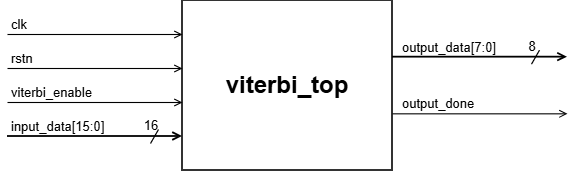
\includegraphics[width=\textwidth,height=4cm,keepaspectratio]{Images/block_diagram/viterbi_top_block_diagram.png}%
}{%
  \fbox{\parbox[c][4cm][c]{.9\textwidth}{\centering\small
    \code{\detokenize{Images/block_diagram/viterbi_top_block_diagram.png}}}}%
}
\caption{Các cổng vào và ra của \code{viterbi\_top}}
\label{fig:top-interface}
\end{figure}

\begin{figure}[H]\centering
% Tai anh len thu muc Images voi dung ten ben duoi.
\IfFileExists{Images/architecture/viterbi_top_architecture.png}{%
  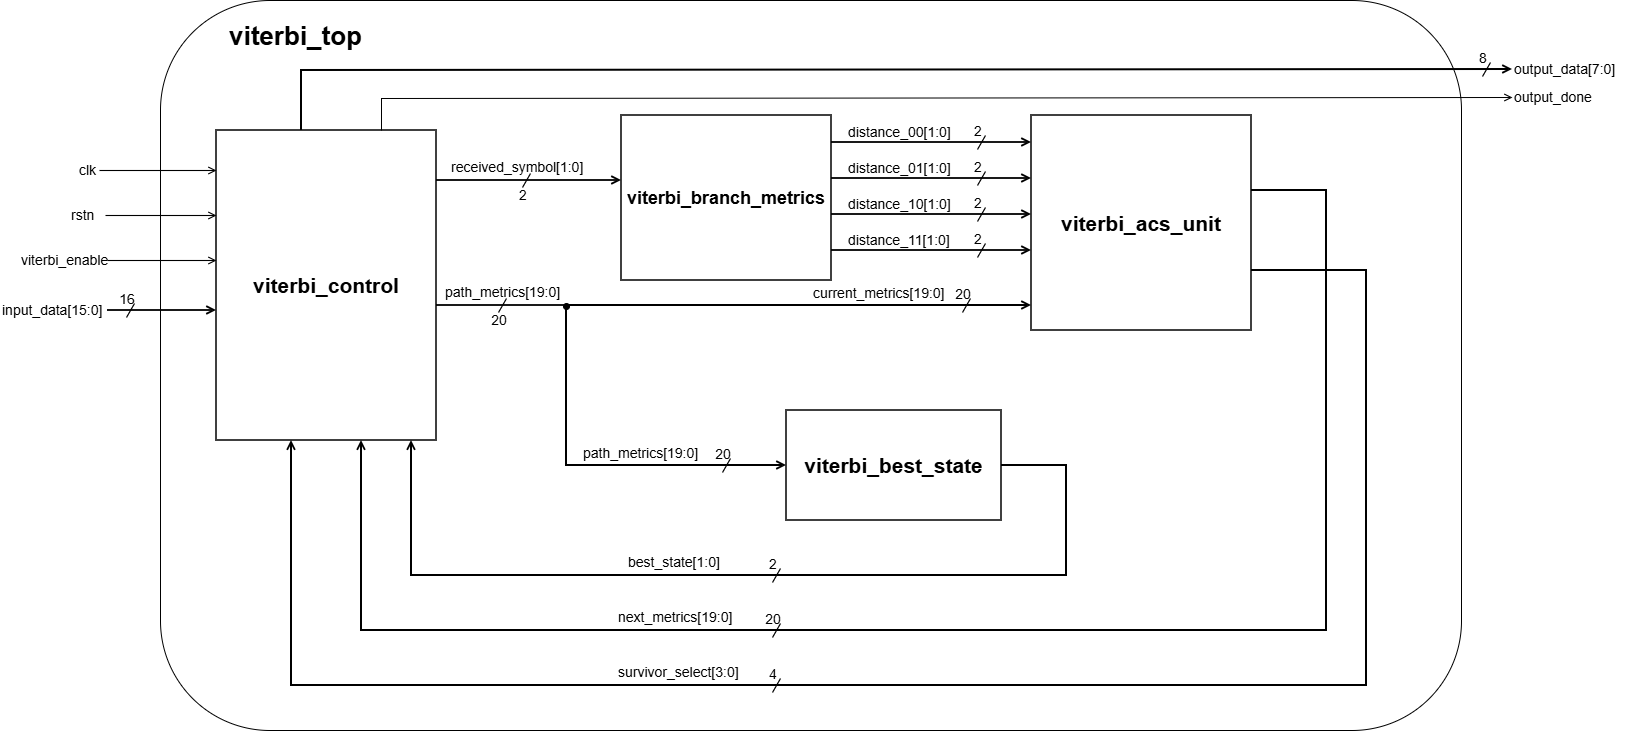
\includegraphics[width=\textwidth,height=10cm,keepaspectratio]{Images/architecture/viterbi_top_architecture.png}%
}{%
  \fbox{\parbox[c][10cm][c]{.9\textwidth}{\centering\small
    \code{\detokenize{Images/architecture/viterbi_top_architecture.png}}}}%
}
\caption{Các module và dây nối bên trong \code{viterbi\_top}}
\label{fig:top}
\end{figure}

Bộ giải mã Viterbi sử dụng tín hiệu \code{clk} để đồng bộ hoạt động và \code{rstn} để khởi tạo trạng thái. Khối điều khiển tiếp nhận tín hiệu cho phép giải mã \code{viterbi\_enable} và dữ liệu đầu vào \code{input\_data}, đồng thời cung cấp kết quả giải mã qua \code{output\_data} và báo hiệu hoàn tất qua \code{output\_done}. Ba khối tính toán được thiết kế theo nguyên lý logic tổ hợp, không yêu cầu tín hiệu clock hoặc reset.

\begin{table}[H]
    \centering
    \small
    \begin{tabularx}{\textwidth}{@{}P{4.5cm}P{2cm}Y@{}}
        \toprule
        \textbf{Khối} & \textbf{Loại mạch} & \textbf{Chức năng} \\
        \midrule

        \texttt{viterbi\_top}
        & Liên kết
        & Cung cấp giao diện vào/ra của bộ giải mã và kết nối khối
          điều khiển với ba khối tính toán. \\

        \texttt{viterbi\_control}
        & Tuần tự và tổ hợp
        & Tiếp nhận và lưu khung dữ liệu đầu vào, điều khiển các bước
          giải mã và truy vết. Khối lưu metric đường đi, quyết định
          chọn đường và kết quả giải mã. \\

        \texttt{viterbi\_branch\_metrics}
        & Tổ hợp
        & Tính khoảng cách Hamming giữa cặp bit nhận được và từng cặp
          bit tham chiếu \texttt{00}, \texttt{01}, \texttt{10},
          \texttt{11} để xác định metric nhánh. \\

        \texttt{viterbi\_acs\_unit}
        & Tổ hợp
        & Cập nhật đồng thời metric đường đi và quyết định chọn đường
          cho cả bốn trạng thái ở mỗi bước của lưới trellis. \\

        \texttt{viterbi\_acs}
        & Tổ hợp
        & Với mỗi đường trong hai đường đi vào cùng một trạng thái,
          cộng metric của trạng thái trước với metric nhánh tương ứng
          và giới hạn tổng ở mức~31. So sánh hai tổng để chọn đường
          có metric nhỏ nhất. \\

        \texttt{viterbi\_best\_state}
        & Tổ hợp
        & Chọn trạng thái có metric đường đi nhỏ nhất ở bước cuối
          của lưới trellis làm điểm bắt đầu truy vết. \\

        \bottomrule
    \end{tabularx}
    \caption{Chức năng của các khối trong bộ giải mã Viterbi}
    \label{tab:modules}
\end{table}

Ở mỗi bước giải mã, khối điều khiển cung cấp một cặp bit nhận được
qua tín hiệu \texttt{received\_symbol}. Khối tính metric nhánh xác định
khoảng cách Hamming giữa cặp bit này và từng cặp bit tham chiếu
\texttt{00}, \texttt{01}, \texttt{10}, \texttt{11}.
Với mỗi trạng thái đích, khối cộng--so sánh--chọn (ACS) sử dụng
metric nhánh và metric đường đi hiện tại để xác định metric mới
và chọn một trong hai đường đi vào trạng thái đó. Phép tính metric
nhánh và phép tính ACS được thực hiện trong cùng một chu kỳ, không
qua thanh ghi trung gian. Tại cạnh lên kế tiếp của \texttt{clk},
khối điều khiển lưu bốn metric mới và bốn bit chọn đường của bước này.

Sau bước thứ tám, khối chọn trạng thái cuối so sánh bốn metric
đường đi đã cập nhật. Khối điều khiển chốt trạng thái có metric
nhỏ nhất làm điểm bắt đầu truy vết. Từ trạng thái này, khối điều
khiển lần lượt đọc các quyết định chọn đường từ bước thứ tám về
bước thứ nhất để khôi phục chuỗi tám bit và xuất kết quả qua
\texttt{output\_data}.

\begin{table}[H]
    \centering
    \small
    \begin{tabularx}{\textwidth}{@{}l c Y@{}}
        \toprule
        \textbf{Tín hiệu} & \textbf{Độ rộng} & \textbf{Ý nghĩa} \\
        \midrule
        \texttt{received\_symbol}
        & 2 bit
        & Cặp bit đầu vào tại bước giải mã hiện tại. \\

        \texttt{distance\_00}, \texttt{distance\_01}
        & 2 bit/tín hiệu
        & Khoảng cách Hamming từ cặp bit đầu vào đến
          \texttt{00} và \texttt{01}, tương ứng. \\

        \texttt{distance\_10}, \texttt{distance\_11}
        & 2 bit/tín hiệu
        & Khoảng cách Hamming từ cặp bit đầu vào đến
          \texttt{10} và \texttt{11}, tương ứng. \\

        \texttt{path\_metrics}
        & 20 bit
        & Bốn metric đường đi hiện tại. Khối ACS dùng các giá trị này
          để cập nhật metric. Sau bước cuối, khối chọn trạng thái
          dùng chúng để xác định điểm bắt đầu truy vết. \\

        \texttt{next\_metrics}
        & 20 bit
        & Bốn metric đường đi mới do khối ACS tính cho bước hiện tại. \\

        \texttt{survivor\_select}
        & 4 bit
        & Bốn bit chọn đường do khối ACS xác định, mỗi bit ứng với
          một trạng thái đích. \\

        \texttt{best\_state}
        & 2 bit
        & Mã trạng thái được chọn để bắt đầu truy vết. \\
        \bottomrule
    \end{tabularx}
    \caption{Các tín hiệu nội bộ của bộ giải mã Viterbi}
    \label{tab:top-wires}
\end{table}

Hai bus \texttt{path\_metrics} và \texttt{next\_metrics} dùng cùng
một quy ước sắp xếp. Mỗi trạng thái chiếm một trường 5 bit trên
mỗi bus và tương ứng với một bit trên \texttt{survivor\_select},
như quy định trong Bảng~\ref{tab:metric-layout}.

\begin{table}[H]
    \centering
    \small
    \begin{tabular}{@{}c c c@{}}
        \toprule
        \textbf{Trạng thái} &
        \textbf{Dải bit trên mỗi bus metric} &
        \textbf{Bit chọn đường} \\
        \midrule
        \texttt{00} & \texttt{[4:0]}   & \texttt{survivor\_select[0]} \\
        \texttt{01} & \texttt{[9:5]}   & \texttt{survivor\_select[1]} \\
        \texttt{10} & \texttt{[14:10]} & \texttt{survivor\_select[2]} \\
        \texttt{11} & \texttt{[19:15]} & \texttt{survivor\_select[3]} \\
        \bottomrule
    \end{tabular}
    \caption{Vị trí metric và bit chọn đường của từng trạng thái}
    \label{tab:metric-layout}
\end{table}

\subsection{Interface Specification}
\begin{table}[H]\centering\small
\begin{tabularx}{\textwidth}{@{}P{3.3cm}c c Y@{}}\toprule
\textbf{Tín hiệu}&\textbf{Hướng}&\textbf{Số bit}&\textbf{Mô tả}\\\midrule
\code{clk}&Vào&1&Clock hệ thống, tác động tại cạnh lên.\\
\code{rstn}&Vào&1&Reset bất đồng bộ, tích cực mức thấp.\\
\code{viterbi\_enable}&Vào&1&Yêu cầu bắt đầu giải mã; chỉ được nhận khi \code{viterbi\_control} ở IDLE.\\
\code{input\_data}&Vào&16&Khung mã hóa được chốt tại cạnh nhận yêu cầu.\\
\code{output\_data}&Ra&8&Kết quả giải mã; giữ đến kết quả tiếp theo hoặc khi reset.\\
\code{output\_done}&Ra&1&Xung một chu kỳ, lên 1 cùng lúc chốt kết quả mới.\\
\bottomrule\end{tabularx}
\caption{I/O table của \code{viterbi\_top}}\label{tab:top-ports}
\end{table}


\subsection{Functional Description}

\subsubsection{Nhận khung và trả kết quả}

Khi \texttt{rstn} ở mức~1, bộ giải mã nhận khung tại cạnh lên của
\texttt{clk} nếu đang ở trạng thái chờ và \texttt{viterbi\_enable}
ở mức~1. Tại cạnh này, bộ giải mã lấy mẫu \texttt{input\_data},
khởi tạo các metric đường đi và bắt đầu giải mã.

Để gửi mỗi khung đúng một lần,
bên gửi đưa \texttt{viterbi\_enable} lên mức~1 trong một chu kỳ và
chờ \texttt{output\_done} trước khi gửi khung tiếp theo. Bộ giải mã
bỏ qua các yêu cầu xuất hiện trong giai đoạn giải mã hoặc truy vết
và không lưu các yêu cầu này để xử lý sau.

Tại cạnh lên hoàn tất truy vết, bộ giải mã đưa kết quả 8 bit lên
\texttt{output\_data} và đặt \texttt{output\_done} lên mức~1 trong
một chu kỳ. Bộ giải mã có thể nhận khung kế tiếp ngay tại cạnh lên
kết thúc xung \texttt{output\_done}. Nếu bên gửi giữ
\texttt{viterbi\_enable} liên tục ở mức~1, bộ giải mã sẽ lấy mẫu
\texttt{input\_data} tại cạnh này, kể cả khi bus vẫn chứa dữ liệu
của khung trước.

\subsubsection{Đáp ứng theo xung nhịp và tín hiệu đặt lại}

Tín hiệu \texttt{rstn} là tín hiệu đặt lại bất đồng bộ, tích cực
ở mức thấp và có ưu tiên cao nhất. Khi \texttt{rstn} ở mức~1,
các điều kiện trong Bảng~\ref{tab:top-priority} được xét theo
trạng thái của bộ giải mã ngay trước cạnh lên của \texttt{clk}.

\begin{table}[H]
    \centering
    \small
    \begin{tabularx}{\textwidth}{@{}P{4.5cm}Y@{}}
        \toprule
        \textbf{Điều kiện} & \textbf{Đáp ứng của bộ giải mã} \\
        \midrule

        \texttt{rstn} ở mức~0
        & Hủy khung đang xử lý, trở về trạng thái chờ và đưa cả
          \texttt{output\_data} lẫn \texttt{output\_done} về~0
          ngay khi tín hiệu đặt lại có hiệu lực. \\

        Đang chờ, \texttt{viterbi\_enable} ở mức~1
        & Nhận khung mới và bắt đầu giải mã. Giữ nguyên
          \texttt{output\_data} và đặt \texttt{output\_done} bằng~0. \\

        Đang chờ, \texttt{viterbi\_enable} ở mức~0
        & Tiếp tục chờ. Giữ nguyên \texttt{output\_data}
          và đặt \texttt{output\_done} bằng~0. \\

        Đang giải mã hoặc thực hiện bước truy vết chưa phải bước cuối
        & Tiếp tục xử lý khung hiện tại. Giữ nguyên \texttt{output\_data}
          và duy trì \texttt{output\_done} ở mức~0. \\

        Thực hiện bước truy vết cuối cùng
        & Ghi kết quả đầy đủ 8 bit lên \texttt{output\_data},
          đặt \texttt{output\_done} bằng~1 và trở về trạng thái chờ. \\

        \bottomrule
    \end{tabularx}
    \caption{Đáp ứng của bộ giải mã khi đặt lại và tại cạnh lên của xung nhịp}
    \label{tab:top-priority}
\end{table}

Bên nhận chỉ ghi nhận kết quả mới khi \texttt{output\_done} ở mức~1.
Giá trị~0 trên \texttt{output\_data} ngay sau khi nhả đặt lại là
giá trị khởi tạo. Sau khi một khung hoàn tất, \texttt{output\_data}
giữ kết quả của khung đó cho đến khi có kết quả mới hoặc khi
\texttt{rstn} trở về mức~0. Mục~\ref{sec:controller} mô tả các
trạng thái điều khiển tương ứng với từng giai đoạn xử lý.

\subsection{Timing}
Gọi $N$ là cạnh lên nhận khung. Bảng~\ref{tab:timing} ghi các công việc theo từng pha. Trạng thái trong bảng là trạng thái trước cạnh lên, tức nhánh được thực hiện tại cạnh đó trong RTL.

\begin{table}[H]\centering\small
\begin{tabularx}{\textwidth}{@{}P{2.2cm}P{3.8cm}Y@{}}\toprule
\textbf{Cạnh clock}&\textbf{Trạng thái trước cạnh}&\textbf{Công việc tại cạnh}\\\midrule
$N$&IDLE&Chốt khung, khởi tạo metric, chuyển sang DECODE.\\
$N+1$ đến $N+8$&DECODE&Cập nhật metric và ghi survivor cho tám symbol, chỉ số từ 0 đến 7.\\
$N+9$&SELECT\_FINAL\_STATE&Chốt \code{best\_state}, đặt chỉ số truy vết bằng 7, chuyển sang TRACEBACK.\\
$N+10$ đến $N+16$&TRACEBACK&Khôi phục bảy bit, từ chỉ số 7 xuống 1.\\
$N+17$&TRACEBACK&Khôi phục bit ở chỉ số 0, chốt \code{output\_data}, đặt \code{output\_done=1}, về IDLE.\\
$N+18$&IDLE&Xóa \code{output\_done}; nhận khung tiếp theo nếu \code{viterbi\_enable=1}.\\
\bottomrule\end{tabularx}
\caption{Thời gian xử lý một khung}\label{tab:timing}
\end{table}

Hình~\ref{fig:viterbi-waveform} minh họa trường hợp gửi hai khung
liên tiếp khi \texttt{rstn} được giữ ở mức~1. Các mốc $N+k$ biểu thị
cạnh lên thứ $k$ tính từ cạnh nhận khung đầu tiên tại $N$. Bảng trên
ghi trạng thái trước mỗi cạnh, còn hàng trạng thái trên hình biểu diễn
trạng thái ngay sau cạnh đó.

\begin{figure}[htbp]
    \centering
    \IfFileExists{Images/waveform/waveform_top_architecture.png}{%
        \includegraphics[width=\linewidth]{Images/waveform/waveform_top_architecture.png}%
    }{%
        \resizebox{\linewidth}{!}{%
        \begin{tikzpicture}[x=1.7cm,y=.65cm,font=\small]
        \foreach \x/\t in {0/{N},1/{N+8},2/{N+9},3/{N+17},4/{N+18}} {
            \draw[gray,densely dotted] (\x,0)--(\x,4.3);
            \node[above] at (\x,4.3) {$\t$};
        }
        \node[left] at (-.35,3.5) {\texttt{viterbi\_enable}};
        \draw[thick] (-.35,3.25)--(-.15,3.25)--(-.15,3.8)--(.15,3.8)--(.15,3.25)--(3.85,3.25)--(3.85,3.8)--(4.15,3.8)--(4.15,3.25)--(4.9,3.25);
        \node[left] at (-.35,2.4) {Trạng thái};
        \foreach \x/\st in {0/DECODE,1/SEL,2/TRACEBACK,3/IDLE,4/DECODE} {
            \draw (\x,2) rectangle ++(1,.8);
            \node[font=\scriptsize] at (\x+.5,2.4) {\st};
        }
        \node[left] at (-.35,1.3) {\texttt{output\_done}};
        \draw[thick] (-.35,1)--(3,1)--(3,1.6)--(4,1.6)--(4,1)--(4.9,1);
        \node[left] at (-.35,.25) {\texttt{output\_data}};
        \draw (0,-.1) rectangle (3,.6) (3,-.1) rectangle (5,.6);
        \node at (1.5,.25) {Kết quả trước}; \node at (4,.25) {Kết quả khung 1};
        \end{tikzpicture}}%
    }
    \caption{Timing diagram khi bộ giải mã nhận hai khung liên tiếp.}
    \label{fig:viterbi-waveform}
\end{figure}

Tại cạnh $N$, bộ giải mã lấy mẫu khung~1 trên \texttt{input\_data}
khi \texttt{viterbi\_enable} ở mức~1. Sau tám bước cập nhật metric,
bộ giải mã chuyển sang trạng thái chọn trạng thái cuối tại cạnh $N+8$
và bắt đầu truy vết sau cạnh $N+9$.

Tại cạnh $N+17$, bộ giải mã xuất kết quả của khung~1 trên
\texttt{output\_data} và đưa \texttt{output\_done} lên mức~1.
Đến cạnh $N+18$, \texttt{output\_done} trở về mức~0. Do
\texttt{viterbi\_enable} đang ở mức~1 tại cạnh này, bộ giải mã
nhận khung~2 trong khi \texttt{output\_data} vẫn giữ kết quả của
khung~1.

Kết quả xuất hiện sau cạnh nhận 17 chu kỳ: tám chu kỳ cập nhật metric, một chu kỳ chọn trạng thái cuối và tám chu kỳ truy vết. Khung tiếp theo được nhận sớm nhất ở $N+18$, vì tại $N+17$ khối vẫn đang thực hiện bước truy vết cuối.

Với clock 200 MHz, 17 chu kỳ tương ứng 85 ns, còn khoảng cách nhận hai khung nhỏ nhất là 90 ns. Thông lượng dữ liệu đã giải mã khi gửi liên tục là
\begin{equation}
T_{\mathrm{info}}=\frac{8}{18}f_{clk}\approx88.89\ \mathrm{Mbit/s}
\quad\text{với } f_{clk}=200\ \mathrm{MHz}.
\end{equation}
\begin{samepage}
Tần số thực tế cần được xác nhận qua báo cáo timing sau tổng hợp và layout. Dữ liệu và enable phải thỏa setup/hold tại cạnh nhận; khi nhả \code{rstn} cần thỏa recovery/removal.

\subsection{Verification Requirements}
Ở mức top, testbench cần kiểm tra dữ liệu giải mã và cách nhận, trả khung. Các trường hợp giao tiếp cần có gồm: enable trong lúc đang xử lý; đổi \code{input\_data} sau cạnh nhận; giữ enable qua lúc hoàn tất; reset giữa khung và gửi lại sau reset. Mỗi lần hoàn tất phải kiểm tra \code{output\_done} xuất hiện đúng tại $N+17$, chỉ dài một chu kỳ, và \code{output\_data} giữ nguyên đến kết quả tiếp theo hoặc reset.



\end{samepage}

\clearpage
\section{ĐẶC TẢ MODULE \code{viterbi\_control}}\label{sec:controller}
\subsection{Overview \& Scope}
\code{viterbi\_control} nhận khung, giữ path metric và survivor, điều khiển tám bước giải mã rồi truy vết để trả byte kết quả. Khối chứa FSM và toàn bộ phần lưu trữ của decoder. Các phép tính branch metric, ACS và chọn metric nhỏ nhất do ba module tổ hợp bên ngoài thực hiện.

\subsection{Architecture}
Hình~\ref{fig:control-block-diagram} là block diagram của \code{viterbi\_control}, thể hiện tên, hướng và độ rộng các cổng vào/ra.

\begin{figure}[H]\centering
% Tai anh block diagram tong cua module len Images voi dung ten file nay.
\IfFileExists{Images/block_diagram/viterbi_control_block_diagram.png}{%
  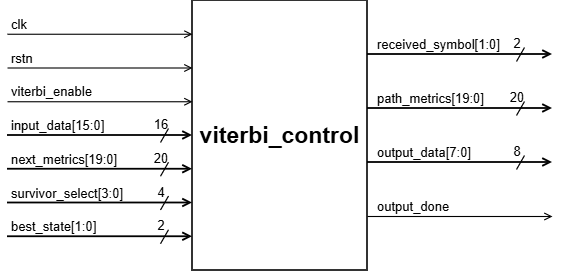
\includegraphics[width=\textwidth,height=6cm,keepaspectratio]{Images/block_diagram/viterbi_control_block_diagram.png}%
}{%
  \fbox{\parbox[c][6cm][c]{.92\textwidth}{\centering\small
    \code{\detokenize{Images/block_diagram/viterbi_control_block_diagram.png}}}}%
}
\caption{Block diagram của \code{viterbi\_control}}\label{fig:control-block-diagram}
\end{figure}

Kiến trúc chi tiết bên trong module được trình bày dưới đây.

Instance \code{control} nằm trong \code{viterbi\_top}. Các tín hiệu trao đổi với ba khối tổ hợp được nối như sau: \code{received\_symbol[1:0]} đi đến \code{viterbi\_branch\_metrics}; \code{path\_metrics[19:0]} đi đến \code{viterbi\_acs\_unit} và \code{viterbi\_best\_state}. Ba đường về là \code{next\_metrics[19:0]}, \code{survivor\_select[3:0]} và \code{best\_state[1:0]}.

\begin{figure}[H]\centering
% Thay anh trong Images de cap nhat so do; khong ve bang TikZ.
\IfFileExists{Images/architecture/viterbi_control_architecture.png}{%
  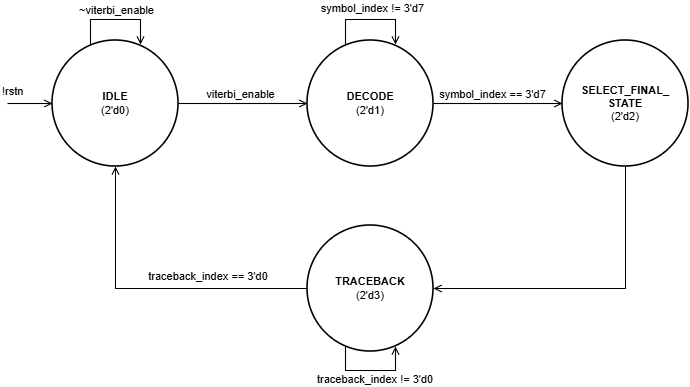
\includegraphics[width=\linewidth,height=8cm,keepaspectratio]{Images/architecture/viterbi_control_architecture.png}%
}{%
  \fbox{\parbox[c][8cm][c]{.92\linewidth}{\centering\small
    \code{\detokenize{Images/architecture/viterbi_control_architecture.png}}}}%
}
\caption{Kiến trúc và các cổng của \code{viterbi\_control}}\label{fig:control-architecture}
\end{figure}


\subsection{Interface Specification}
\begin{table}[H]\centering\small
\begin{tabularx}{\textwidth}{@{}P{3.5cm}c c Y@{}}\toprule
\textbf{Cổng}&\textbf{Hướng}&\textbf{Số bit}&\textbf{Mô tả}\\\midrule
\code{clk}&Vào&1&Clock cạnh lên.\\
\code{rstn}&Vào&1&Reset bất đồng bộ, tích cực mức thấp.\\
\code{viterbi\_enable}&Vào&1&Nhận khung khi FSM ở IDLE.\\
\code{input\_data}&Vào&16&Khung mã hóa, chốt tại cạnh nhận yêu cầu.\\
\code{next\_metrics}&Vào&20&Bốn metric mới từ \code{viterbi\_acs\_unit}.\\
\code{survivor\_select}&Vào&4&Bốn decision từ \code{viterbi\_acs\_unit}.\\
\code{best\_state}&Vào&2&Mã trạng thái có metric nhỏ nhất từ \code{viterbi\_best\_state}.\\
\code{received\_symbol}&Ra&2&Nối trực tiếp với \code{encoded\_shift[15:14]}.\\
\code{path\_metrics}&Ra&20&Metric hiện tại, đóng gói $\{PM11,PM10,PM01,PM00\}$.\\
\code{output\_done}&Ra&1&Xung một chu kỳ khi chốt kết quả.\\
\code{output\_data}&Ra&8&Byte kết quả, giữ đến lần hoàn tất tiếp theo hoặc reset.\\
\bottomrule\end{tabularx}
\caption{I/O table của \code{viterbi\_control}}\label{tab:control-ports}
\end{table}
Không có cổng valid/ready riêng với các khối tổ hợp. Controller dùng trạng thái FSM để quyết định lúc chốt metric, decision hoặc trạng thái cuối. Khối không có cổng \code{busy} và không có tham số chọn chiều đọc symbol.


\subsection{Functional Description}
FSM điều khiển một khung qua bốn trạng thái như Hình~\ref{fig:fsm}. Khi \texttt{rstn=1}, điều kiện chuyển trạng thái được xét tại cạnh lên của \texttt{clk}, theo giá trị chỉ số và tín hiệu trước cạnh. Nếu \texttt{rstn} xuống mức~0 ở bất kỳ trạng thái nào, bộ điều khiển hủy khung đang xử lý, về \texttt{IDLE} và đưa cả \texttt{output\_done} lẫn \texttt{output\_data} về~0 ngay lập tức.

\begin{figure}[H]\centering
\begin{tikzpicture}[>=Stealth,thick,
 st/.style={draw,rounded corners,minimum height=1cm,minimum width=3.4cm,font=\small\ttfamily},
 lab/.style={font=\footnotesize,align=center,fill=white,inner sep=2pt}]
\node[st] (i) at (0,0) {IDLE};
\node[st] (d) at (7,0) {DECODE};
\node[st] (s) at (7,-3) {SELECT\_FINAL\_STATE};
\node[st] (t) at (0,-3) {TRACEBACK};
\draw[->] (i) -- node[lab,above]{\texttt{enable=1}} (d);
\draw[->] (d) -- node[lab,right]{chỉ số symbol $=7$} (s);
\draw[->] (s) -- node[lab,above]{cạnh kế tiếp} (t);
\draw[->] (t) -- node[lab,right]{chỉ số truy vết $=0$} (i);
\draw[->] (i) edge[loop above] node[lab,above]{\texttt{enable=0}} (i);
\draw[->] (d) edge[loop above] node[lab,above]{chỉ số symbol $<7$} (d);
\draw[->] (t) edge[loop below] node[lab,below]{chỉ số truy vết $>0$} (t);
\draw[->] (-3,0) -- node[lab,above]{reset} (i);
\end{tikzpicture}
\caption{Sơ đồ trạng thái của bộ điều khiển}\label{fig:fsm}
\end{figure}

Bảng~\ref{tab:control-fsm-transitions} tóm tắt hoạt động của FSM khi \texttt{rstn=1}. Hai cột đầu ghi trạng thái và điều kiện ngay trước cạnh lên của \texttt{clk}. Hai cột sau ghi trạng thái kế tiếp và thao tác thực hiện tại cạnh đó. Trong bảng, \texttt{SEL} là \texttt{SELECT\_FINAL\_STATE}, $k$ là \texttt{symbol\_index} và $t$ là \texttt{traceback\_index}.

\begin{table}[H]
    \centering\small
    \setlength{\tabcolsep}{4pt}
    \begin{tabularx}{\linewidth}{@{}l P{2.7cm} l Y@{}}
        \toprule
        \textbf{Trước cạnh} & \textbf{Điều kiện} & \textbf{Sau cạnh} & \textbf{Thao tác tại cạnh lên} \\
        \midrule
        \texttt{IDLE} & \texttt{viterbi\_enable} bằng~0 & \texttt{IDLE}
        & Tiếp tục chờ, giữ byte kết quả trên \texttt{output\_data}. \\
        \texttt{IDLE} & \texttt{viterbi\_enable} bằng~1 & \texttt{DECODE}
        & Nhận khung từ \texttt{input\_data}, khởi tạo metric các trạng thái $(00,01,10,11)$ thành $(0,31,31,31)$, đặt $k=0$ và xóa byte đang khôi phục. \\
        \texttt{DECODE} & $0\leq k<7$ & \texttt{DECODE}
        & Chốt bốn metric mới, ghi bốn bit chọn đường vào hàng $k$, dịch khung sang trái hai bit và tăng $k$ một đơn vị. \\
        \texttt{DECODE} & $k=7$ & \texttt{SEL}
        & Chốt bốn metric cuối, ghi bốn bit chọn đường vào hàng~7 và dịch khung lần cuối. Chỉ số $k$ giữ ở~7. \\
        \texttt{SEL} & Cạnh lên kế tiếp & \texttt{TRACEBACK}
        & Chốt \texttt{best\_state} làm trạng thái bắt đầu truy vết và đặt $t=7$. \\
        \texttt{TRACEBACK} & $0<t\leq 7$ & \texttt{TRACEBACK}
        & Ghi bit cao của trạng thái truy vết vào vị trí $7-t$ của byte đang khôi phục. Chuyển về trạng thái trước theo quyết định ở hàng $t$ và giảm $t$ một đơn vị. \\
        \texttt{TRACEBACK} & $t=0$ & \texttt{IDLE}
        & Ghi bit cuối vào vị trí~7, chốt byte đầy đủ lên \texttt{output\_data} và đặt \texttt{output\_done} lên~1. Cập nhật trạng thái truy vết theo quyết định ở hàng~0. \\
        \bottomrule
    \end{tabularx}
    \caption{Điều kiện chuyển trạng thái và thao tác của bộ điều khiển}
    \label{tab:control-fsm-transitions}
\end{table}

Chỉ cạnh hoàn tất truy vết đặt \texttt{output\_done} lên~1. Ở sáu trường hợp còn lại, tín hiệu này bằng~0 sau cạnh lên. Reset bất đồng bộ có ưu tiên cao hơn mọi điều kiện trong bảng.

\subsubsection{\texttt{IDLE} (00) --- Chờ nhận khung}
\textbf{Ý nghĩa và điều kiện vào.} FSM vào trạng thái chờ sau reset hoặc tại cạnh hoàn tất bước truy vết cuối. Bộ điều khiển chỉ nhận khung mới khi đang ở trạng thái này.

\textbf{Đầu ra.} Sau reset, \texttt{output\_data} và \texttt{output\_done} đều bằng~0. Khi trở về từ \texttt{TRACEBACK}, \texttt{output\_data} chứa byte vừa giải mã và \texttt{output\_done} bằng~1 trong chu kỳ đầu ở \texttt{IDLE}. Tại cạnh lên kế tiếp, \texttt{output\_done} về~0, kể cả khi nhận ngay khung mới.

\textbf{Điều kiện ra.} Nếu \texttt{viterbi\_enable=0}, FSM tiếp tục chờ và giữ byte kết quả. Nếu \texttt{viterbi\_enable=1} tại cạnh lên, bộ điều khiển chốt khung 16 bit trên \texttt{input\_data} và chuyển sang \texttt{DECODE}.

\subsubsection{\texttt{DECODE} (01) --- Xử lý tám symbol}
\textbf{Ý nghĩa và điều kiện vào.} FSM vào \texttt{DECODE} tại cạnh nhận khung. Chỉ số symbol bắt đầu từ~0. Vì khung bắt đầu tại trạng thái trellis \texttt{00}, metric ban đầu của các trạng thái $(00,01,10,11)$ lần lượt là $(0,31,31,31)$.

\textbf{Đầu ra và thao tác.} Ngay sau cạnh nhận khung, \texttt{received\_symbol} mang cặp bit \texttt{input\_data[15:14]} và \texttt{path\_metrics} mang bộ metric ban đầu. Tại mỗi cạnh lên trong \texttt{DECODE}, bộ điều khiển cập nhật \texttt{path\_metrics} từ \texttt{next\_metrics} và lưu bốn bit \texttt{survivor\_select} vào hàng mang chỉ số symbol hiện tại. Các cặp bit được xử lý lần lượt từ cao xuống thấp. \texttt{output\_done} bằng~0 và \texttt{output\_data} giữ nguyên.

\textbf{Điều kiện ra.} Với \texttt{symbol\_index} từ~0 đến~6, FSM tăng chỉ số một đơn vị và ở lại \texttt{DECODE}. Khi chỉ số trước cạnh bằng~7, bộ điều khiển chốt kết quả của symbol thứ tám rồi chuyển sang \texttt{SELECT\_FINAL\_STATE} ngay tại cạnh đó.

\subsubsection{\texttt{SELECT\_FINAL\_STATE} (10) --- Chọn điểm bắt đầu truy vết}
\textbf{Ý nghĩa và điều kiện vào.} FSM vào trạng thái này sau khi đã chốt đủ tám lần cập nhật metric. Một chu kỳ được dành cho khối chọn trạng thái xác định \texttt{best\_state} từ bộ metric cuối.

\textbf{Đầu ra.} \texttt{path\_metrics} giữ bốn metric cuối để khối chọn trạng thái so sánh. \texttt{output\_done} bằng~0 và \texttt{output\_data} giữ nguyên.

\textbf{Điều kiện ra.} Tại cạnh lên kế tiếp, bộ điều khiển chốt \texttt{best\_state} vào \texttt{traceback\_state}, đặt \texttt{traceback\_index} bằng~7 và chuyển sang \texttt{TRACEBACK}.

\subsubsection{\texttt{TRACEBACK} (11) --- Khôi phục byte kết quả}\label{sec:control-traceback}
\textbf{Ý nghĩa và điều kiện vào.} FSM vào \texttt{TRACEBACK} khi đã chốt trạng thái cuối và chỉ số~7. Mỗi cạnh lên xử lý một hàng quyết định, theo thứ tự từ hàng~7 về hàng~0.

\textbf{Đầu ra và thao tác.} Với chỉ số hiện tại $t$, bit cao của \texttt{traceback\_state} là bit thông tin được ghi vào vị trí $7-t$ trong byte đang khôi phục. Bit quyết định đã lưu cho trạng thái hiện tại ở hàng $t$ xác định trạng thái trước. Trong bảy bước đầu, \texttt{output\_done=0} và \texttt{output\_data} giữ byte kết quả trước đó.

\textbf{Điều kiện ra.} Nếu $t>0$, bộ điều khiển giảm chỉ số một đơn vị và tiếp tục truy vết. Nếu $t=0$, bộ điều khiển ghép bit cuối vào vị trí~7, chốt byte đầy đủ lên \texttt{output\_data}, đặt \texttt{output\_done=1} và về \texttt{IDLE} tại cùng cạnh lên. Các yêu cầu nhận khung xuất hiện khi đang giải mã, chọn trạng thái cuối hoặc truy vết đều bị bỏ qua.

\subsection{Timing}
Gọi $N$ là cạnh controller nhận khung. Các dữ liệu từ khối tổ hợp phải ổn định trước cạnh lấy mẫu tương ứng.
\begin{table}[H]\centering\small
\begin{tabularx}{\textwidth}{@{}P{2.4cm}P{4cm}Y@{}}\toprule
\textbf{Cạnh}&\textbf{Dữ liệu được chốt}&\textbf{Thao tác sau cạnh}\\\midrule
$N$&\code{input\_data}&Giữ khung, khởi tạo metric, bắt đầu DECODE.\\
$N+1$ đến $N+8$&\code{next\_metrics}, \code{survivor\_select}&Cập nhật metric và ghi survivor, mỗi cạnh một symbol.\\
$N+9$&\code{best\_state}&Nạp trạng thái truy vết và chỉ số 7.\\
$N+10$ đến $N+16$&\code{decoded\_next}&Khôi phục bảy bit vào các vị trí [0] đến [6].\\
$N+17$&\code{decoded\_next}&Ghi bit [7], chốt \code{output\_data}, phát \code{output\_done}.\\
$N+18$&Khung mới nếu enable bằng 1&Xóa xung hoàn tất; có thể nhận khung kế tiếp.\\
\bottomrule\end{tabularx}
\caption{Các cạnh lấy mẫu của controller}\label{tab:control-timing}
\end{table}
\begin{figure}[H]\centering
% Thay anh trong Images de cap nhat so do; khong ve bang TikZ.
\IfFileExists{Images/waveform/waveform_viterbi_control.png}{%
  \includegraphics[width=\linewidth,height=5cm,keepaspectratio]{Images/waveform/waveform_viterbi_control.png}%
}{%
  \fbox{\parbox[c][5cm][c]{.92\linewidth}{\centering\small
    \code{\detokenize{Images/waveform/waveform_viterbi_control.png}}}}%
}
\caption{Timing của các pha và các lần cập nhật thanh ghi trong controller}\label{fig:control-waveform}
\end{figure}


Khi nhả \code{rstn}, cần thỏa recovery/removal. Reset đang được giữ ở mức 0 phải ưu tiên hơn enable hoặc thao tác ghi kết quả.


\subsection{Verification Requirements}
Với khung nhận tại cạnh $N$, kiểm tra tám lần cập nhật metric tại $N+1$ đến $N+8$, một lần chốt trạng thái cuối tại $N+9$ và tám bước truy vết tại $N+10$ đến $N+17$. Xung \texttt{output\_done} phải trùng với lần cập nhật byte kết quả tại $N+17$. Kiểm tra thêm việc nhận khung kế tiếp tại $N+18$, bỏ qua yêu cầu khi đang xử lý và hủy khung khi reset ở từng pha.

\clearpage
\section{ĐẶC TẢ MODULE \texttt{viterbi\_branch\_metrics}}
\label{sec:bmu}

\subsection{Overview \& Scope}

Tại mỗi bước giải mã, bộ giải mã Viterbi cần đánh giá mức độ phù hợp
giữa cặp bit nhận được và nhãn mã hóa của từng nhánh trên trellis.
Khối tính metric nhánh (Branch Metric Unit, BMU) thực hiện phép đánh
giá này bằng khoảng cách Hamming, tức là số vị trí bit khác nhau giữa
hai cặp bit.

Trellis có tám nhánh nhưng chỉ sử dụng bốn nhãn mã hóa:
\texttt{00}, \texttt{01}, \texttt{10} và \texttt{11}. Vì vậy, với mỗi
cặp bit đầu vào, BMU chỉ cần cung cấp bốn khoảng cách. Các nhánh có
cùng nhãn sử dụng chung một giá trị khi khối ACS cập nhật metric
đường đi.

\subsection{Architecture}

BMU là khối tổ hợp với một đầu vào 2 bit và bốn đầu ra 2 bit.
Như minh họa trong Hình~\ref{fig:bmu}, cả bốn phép tính sử dụng cùng
một cặp bit nhận được. Mỗi phép tính so sánh cặp bit này với một nhãn
tham chiếu cố định và đếm số vị trí khác nhau. Bốn khoảng cách được
cung cấp song song cho khối \texttt{viterbi\_acs\_unit} trong cùng
bước giải mã.

Hình~\ref{fig:bmu-block-diagram} là block diagram của \code{viterbi\_branch\_metrics}, thể hiện tên, hướng và độ rộng các cổng vào/ra.

\begin{figure}[H]\centering
% Tai anh block diagram tong cua module len Images voi dung ten file nay.
\IfFileExists{Images/block_diagram/viterbi_branch_metrics_block_diagram.png}{%
  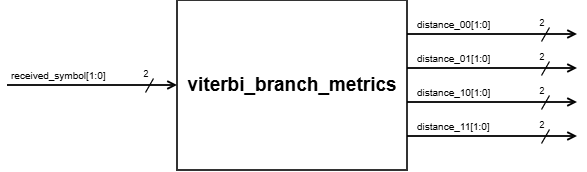
\includegraphics[width=\textwidth,height=6cm,keepaspectratio]{Images/block_diagram/viterbi_branch_metrics_block_diagram.png}%
}{%
  \fbox{\parbox[c][6cm][c]{.92\textwidth}{\centering\small
    \code{\detokenize{Images/block_diagram/viterbi_branch_metrics_block_diagram.png}}}}%
}
\caption{Block diagram của \code{viterbi\_branch\_metrics}}\label{fig:bmu-block-diagram}
\end{figure}

Kiến trúc chi tiết bên trong module được trình bày dưới đây.

\begin{figure}[H]\centering
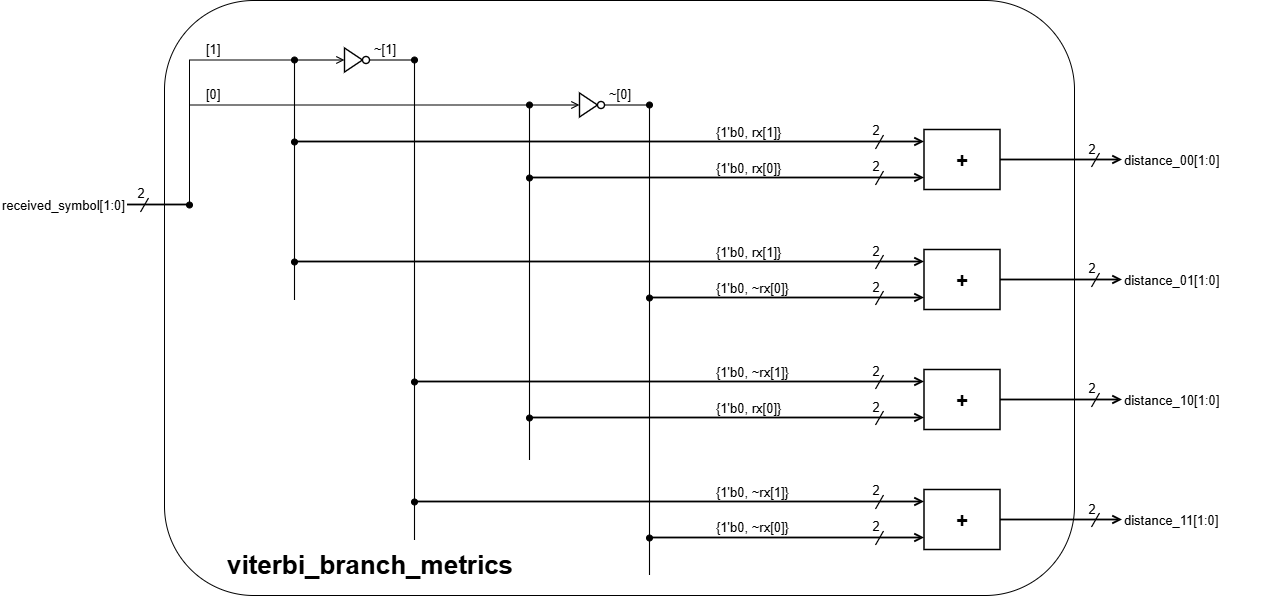
\includegraphics[width=\textwidth,height=.44\textheight,keepaspectratio]{Images/architecture/viterbi_branch_metrics_architecture.png}
\caption{BMU: tính bốn khoảng cách Hamming từ một symbol 2 bit}\label{fig:bmu}
\end{figure}

\subsection{Interface Specification}

Bảng~\ref{tab:bmu-ports} quy định các cổng dữ liệu của BMU. Hai chữ số
trong tên mỗi cổng \texttt{distance} biểu thị nhãn tham chiếu dùng để
tính khoảng cách tại cổng đó.

\begin{table}[H]
    \centering
    \small
    \begin{tabularx}{\textwidth}{@{}l c c Y@{}}
        \toprule
        \textbf{Cổng} & \textbf{Hướng} & \textbf{Độ rộng}
        & \textbf{Ý nghĩa} \\
        \midrule
        \texttt{received\_symbol} & Vào & 2 bit
        & Cặp bit nhận được tại bước giải mã hiện tại.
          Bit~1 là $r_1$, bit~0 là $r_0$. \\
        \texttt{distance\_00} & Ra & 2 bit
        & Khoảng cách Hamming đến nhãn \texttt{00}. \\
        \texttt{distance\_01} & Ra & 2 bit
        & Khoảng cách Hamming đến nhãn \texttt{01}. \\
        \texttt{distance\_10} & Ra & 2 bit
        & Khoảng cách Hamming đến nhãn \texttt{10}. \\
        \texttt{distance\_11} & Ra & 2 bit
        & Khoảng cách Hamming đến nhãn \texttt{11}. \\
        \bottomrule
    \end{tabularx}
    \caption{Giao diện dữ liệu của khối tính metric nhánh}
    \label{tab:bmu-ports}
\end{table}

\subsection{Functional Description}

\subsubsection{Xác định metric nhánh}

Gọi $r=(r_1,r_0)$ là cặp bit nhận được và $v=(v_1,v_0)$ là nhãn
tham chiếu. Tại vị trí $i$, bit sai khác $e_i=r_i\oplus v_i$ bằng~1
khi $r_i$ khác $v_i$. Khoảng cách Hamming $d_v$ bằng tổng số học
của hai bit sai khác:
\begin{equation}
    d_v=e_1+e_0=(r_1\oplus v_1)+(r_0\oplus v_0).
\end{equation}

Với bit tham chiếu bằng~0, bit sai khác bằng chính bit nhận được.
Với bit tham chiếu bằng~1, bit sai khác bằng giá trị đảo của bit
nhận được. Áp dụng quy tắc này cho bốn nhãn, ta có
\begin{equation}
    \begin{aligned}
        d_{00} &= r_1+r_0, &
        d_{01} &= r_1+\overline{r_0}, \\
        d_{10} &= \overline{r_1}+r_0, &
        d_{11} &= \overline{r_1}+\overline{r_0}.
    \end{aligned}
\end{equation}

Bảng~\ref{tab:bmu-truth} quy định giá trị thập phân tại từng đầu ra
cho cả bốn trường hợp đầu vào hợp lệ.

\begin{table}[H]
    \centering
    \small
    \begin{tabular}{@{}ccccc@{}}
        \toprule
        \textbf{Cặp bit nhận} & $d_{00}$ & $d_{01}$ & $d_{10}$ & $d_{11}$ \\
        \midrule
        \texttt{00} & 0 & 1 & 1 & 2 \\
        \texttt{01} & 1 & 0 & 2 & 1 \\
        \texttt{10} & 1 & 2 & 0 & 1 \\
        \texttt{11} & 2 & 1 & 1 & 0 \\
        \bottomrule
    \end{tabular}
    \caption{Giá trị metric nhánh ứng với từng cặp bit nhận được}
    \label{tab:bmu-truth}
\end{table}

Ví dụ, khi nhận \texttt{10}, BMU cho $d_{10}=0$ vì hai bit đều khớp
với nhãn \texttt{10}, và $d_{01}=2$ vì cả hai bit đều khác nhãn
\texttt{01}. Hai nhãn còn lại đều có khoảng cách bằng~1. Các giá trị
này chỉ đánh giá cặp bit ở bước hiện tại. Để chọn đường đi vào mỗi
trạng thái đích, khối ACS cộng metric của từng nhánh với metric đường
đi đã tích lũy tại trạng thái trước tương ứng.

\subsubsection{Biểu diễn kết quả và điều kiện kiểm tra}

Mỗi đầu ra biểu diễn số vị trí sai khác dưới dạng số nhị phân
không dấu 2 bit. Khi cộng $e_1$ và $e_0$, bit thấp của kết quả là
$e_1\oplus e_0$ và bit cao là $e_1\land e_0$. Bảng dưới đây thể hiện
cách mã hóa kết quả, bao gồm trường hợp cả hai vị trí đều sai khác.

\begin{table}[H]
    \centering
    \small
    \begin{tabular}{@{}c c c l@{}}
        \toprule
        $e_1$ & $e_0$ & \textbf{Đầu ra [1:0]} & \textbf{Ý nghĩa} \\
        \midrule
        0 & 0 & \texttt{00} & Khớp cả hai vị trí. \\
        0 & 1 & \texttt{01} & Khác tại vị trí bit~0. \\
        1 & 0 & \texttt{01} & Khác tại vị trí bit~1. \\
        1 & 1 & \texttt{10} & Khác tại cả hai vị trí. \\
        \bottomrule
    \end{tabular}
    \caption{Biểu diễn khoảng cách Hamming trên đầu ra 2 bit}
\end{table}

Với đầu vào nhị phân hợp lệ, mỗi đầu ra chỉ nhận một trong ba giá trị
\texttt{00}, \texttt{01} hoặc \texttt{10}. Ngoài ra, đối với hai nhãn
bù nhau, tại mỗi vị trí, bit nhận được khớp với đúng một trong hai bit
tham chiếu. Do đó, các khoảng cách phải thỏa mãn
\begin{equation}
    d_{00}+d_{11}=2,\qquad d_{01}+d_{10}=2.
\end{equation}

Khi kiểm tra chức năng, cần đối chiếu từng cổng với
Bảng~\ref{tab:bmu-truth}. Hai quan hệ tổng trên giúp kiểm tra tính
nhất quán của các kết quả, nhưng vẫn đúng nếu hoán đổi hai đầu ra
\texttt{distance\_01} và \texttt{distance\_10}. Giá trị đầu ra khi
\texttt{received\_symbol} chứa \texttt{X} hoặc \texttt{Z} nằm ngoài
phạm vi của bảng chân trị.

\subsection{Timing}

BMU không sử dụng xung nhịp hay tín hiệu đặt lại. Khi
\texttt{received\_symbol} thay đổi và ổn định ở một giá trị mới,
bốn đầu ra phải đạt các giá trị tương ứng trong
Bảng~\ref{tab:bmu-truth} sau thời gian lan truyền của mạch tổ hợp.
Hình~\ref{fig:bmu-waveform} minh họa đáp ứng này.

\begin{figure}[H]
    \centering
    \IfFileExists{Images/waveform/waveform_viterbi_branch_metrics.png}{%
        \includegraphics[
            width=\linewidth,
            height=4cm,
            keepaspectratio
        ]{Images/waveform/waveform_viterbi_branch_metrics.png}%
    }{%
        \fbox{\parbox[c][4cm][c]{.92\linewidth}{\centering
            Giản đồ thời gian của khối tính metric nhánh}}%
    }
    \caption{Đáp ứng của bốn đầu ra khoảng cách khi cặp bit nhận thay đổi}
    \label{fig:bmu-waveform}
\end{figure}

Trong một bước giải mã, BMU và ACS phải hoàn thành phép tính trong
cùng một chu kỳ. Yêu cầu thời gian áp dụng cho toàn bộ đường dữ liệu:
từ khi khối điều khiển cung cấp cặp bit nhận được, qua phép tính
khoảng cách và cập nhật metric, đến khi metric mới và các bit chọn
đường đáp ứng thời gian thiết lập trước cạnh lên kế tiếp của
\texttt{clk}. BMU không bổ sung chu kỳ trễ riêng vào lịch giải mã.


\subsection{Verification Requirements}
% TODO: Bo sung yeu cau kiem chung o buoc tiep theo.

\clearpage
\section{ĐẶC TẢ MODULE \texttt{viterbi\_acs}}
\label{sec:acs}

\subsection{Overview \& Scope}

Tại mỗi bước giải mã, có hai đường đi vào cùng một trạng thái đích
trên trellis. Khối cộng--so sánh--chọn (Add--Compare--Select, ACS)
xác định đường được giữ lại bằng cách cộng metric của từng trạng thái
trước với metric của nhánh tương ứng, sau đó so sánh hai kết quả.
Mỗi khối \texttt{viterbi\_acs} thực hiện phép tính này cho một
trạng thái đích.

ACS cung cấp hai kết quả cho cùng một bước giải mã. Đầu ra
\texttt{survivor\_metric} là metric đường đi mới của trạng thái
đích, được dùng trong bước giải mã tiếp theo. Đầu ra
\texttt{survivor\_select} xác định đường đã được chọn để khối
điều khiển lưu quyết định phục vụ truy vết.

\subsection{Architecture}

Hình~\ref{fig:acs-block-diagram} trình bày giao diện của một ACS.
Chỉ số~0 và~1 phân biệt hai đường đi vào trạng thái đích. Metric
của trạng thái trước và metric nhánh phải được ghép theo cùng chỉ số.

\begin{figure}[H]
    \centering
    \IfFileExists{Images/block_diagram/viterbi_acs_block_diagram.png}{%
        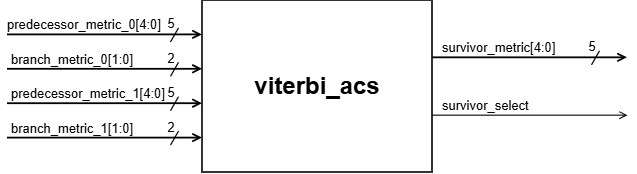
\includegraphics[width=\linewidth,height=6cm,keepaspectratio]
            {Images/block_diagram/viterbi_acs_block_diagram.png}%
    }{%
        \fbox{\parbox[c][4cm][c]{.92\linewidth}{\centering
            Sơ đồ khối \texttt{Images/block_diagram/viterbi_acs_block_diagram.png}}}%
    }
    \caption{Giao diện của khối ACS cho một trạng thái đích}
    \label{fig:acs-block-diagram}
\end{figure}

Hai đường ứng viên được đánh giá song song như trong
Hình~\ref{fig:acs}. Trên mỗi đường, ACS tính tổng metric và giới hạn
kết quả ở giá trị lớn nhất có thể biểu diễn. Hai giá trị sau bão hòa
là đầu vào của phép so sánh. Cùng một quyết định chọn đường xác định
cả metric đầu ra và bit dùng cho truy vết.

\begin{figure}[H]
    \centering
    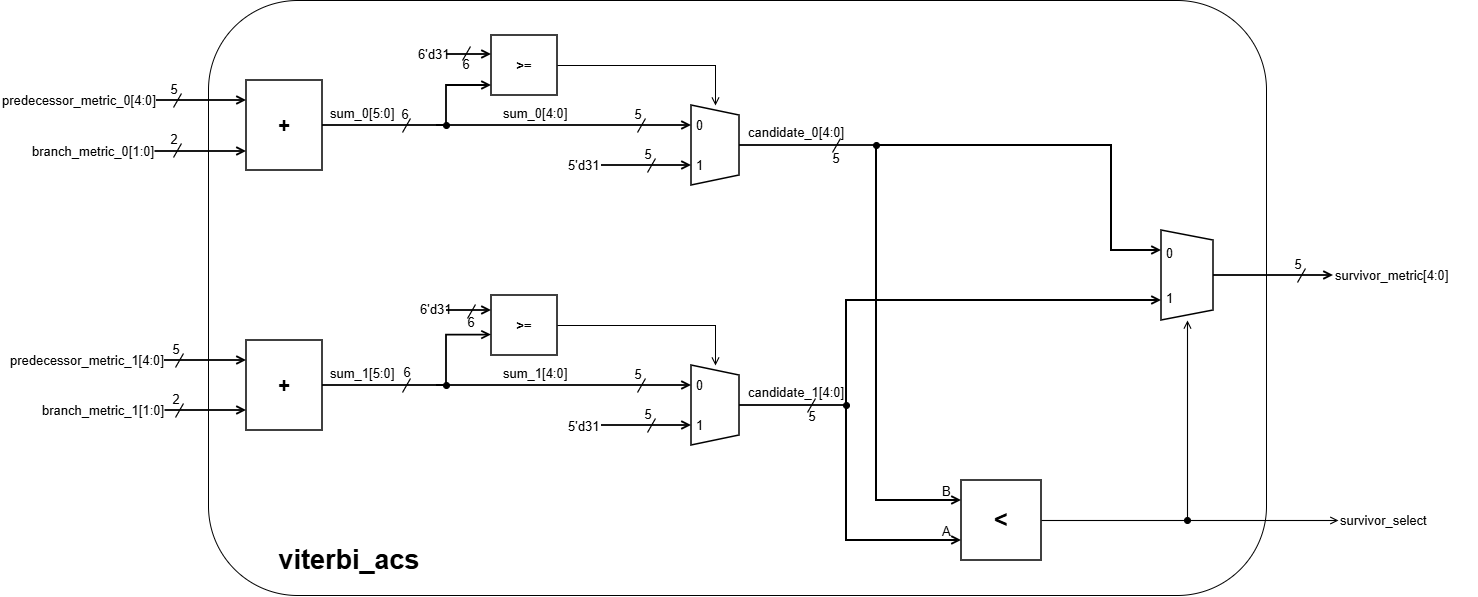
\includegraphics[width=\linewidth,height=.45\textheight,keepaspectratio]
        {Images/architecture/viterbi_acs_architecture.png}
    \caption{Hai đường tính metric và phép chọn đường của ACS}
    \label{fig:acs}
\end{figure}

\begin{table}[H]
    \centering
    \small
    \begin{tabularx}{\textwidth}{@{}l c Y@{}}
        \toprule
        \textbf{Đại lượng} & \textbf{Độ rộng} & \textbf{Ý nghĩa} \\
        \midrule
        Tổng metric mỗi đường & 6 bit
        & Tổng đầy đủ của metric trạng thái trước và metric nhánh,
          bao gồm cả phần vượt quá~31. \\
        Metric ứng viên mỗi đường & 5 bit
        & Giá trị của từng đường sau khi giới hạn tổng ở~31. \\
        Quyết định chọn đường & 1 bit
        & Chỉ số của đường được giữ lại cho trạng thái đích. \\
        Metric đường được chọn & 5 bit
        & Metric ứng viên tương ứng với quyết định chọn đường. \\
        \bottomrule
    \end{tabularx}
    \caption{Các đại lượng trong phép tính ACS ở cấu hình metric 5 bit}
    \label{tab:acs-wires}
\end{table}

\subsection{Interface Specification}

Gọi $W$ là độ rộng metric đường đi, do tham số
\texttt{METRIC\_WIDTH} quy định. Bộ giải mã sử dụng cấu hình
mặc định $W=5$. Các cổng metric mang giá trị nguyên không dấu.
Độ rộng của metric nhánh là 2 bit, độc lập với $W$.

\begin{table}[H]
    \centering
    \small
    \begin{tabularx}{\textwidth}{@{}l c c Y@{}}
        \toprule
        \textbf{Cổng} & \textbf{Hướng} & \textbf{Độ rộng}
        & \textbf{Ý nghĩa} \\
        \midrule
        \texttt{predecessor\_metric\_0} & Vào & $W$ bit
        & Metric đã tích lũy tại trạng thái trước của đường~0. \\
        \texttt{branch\_metric\_0} & Vào & 2 bit
        & Metric của nhánh nối trạng thái trước trên đường~0
          với trạng thái đích. \\
        \texttt{predecessor\_metric\_1} & Vào & $W$ bit
        & Metric đã tích lũy tại trạng thái trước của đường~1. \\
        \texttt{branch\_metric\_1} & Vào & 2 bit
        & Metric của nhánh nối trạng thái trước trên đường~1
          với trạng thái đích. \\
        \texttt{survivor\_metric} & Ra & $W$ bit
        & Metric đường đi mới của trạng thái đích. \\
        \texttt{survivor\_select} & Ra & 1 bit
        & Bằng~0 khi chọn đường~0 và bằng~1 khi chọn đường~1. \\
        \bottomrule
    \end{tabularx}
    \caption{Giao diện dữ liệu của khối ACS}
    \label{tab:acs-ports}
\end{table}

Trong bộ giải mã, mỗi metric nhánh là khoảng cách Hamming giữa hai
cặp bit nên chỉ nhận các giá trị 0, 1 hoặc~2. Mã \texttt{11}
trên cổng metric nhánh biểu diễn giá trị~3 và chỉ dùng khi cần
kiểm tra toàn bộ miền đầu vào của riêng khối ACS.

\subsection{Functional Description}

\subsubsection{Cập nhật metric cho hai đường ứng viên}

Với đường $i\in\{0,1\}$, gọi $PM_i$ là metric của trạng thái trước
và $BM_i$ là metric nhánh tại bước hiện tại. Gọi $M=2^W-1$ là giá trị
lớn nhất biểu diễn được trên cổng metric. Tổng $s_i$ và metric
ứng viên $c_i$ được xác định bởi
\begin{equation}
    s_i=PM_i+BM_i,
    \qquad
    c_i=\min(s_i,M).
\end{equation}

Ở cấu hình $W=5$, ngưỡng $M$ bằng~31. Tổng lớn nhất trong luồng
giải mã là $31+2=33$. Nếu xét cả mã đầu vào \texttt{11} của cổng
metric nhánh, tổng lớn nhất là $31+3=34$. Tổng 6 bit biểu diễn được
đầy đủ cả hai trường hợp trước khi đưa kết quả về miền 5 bit.

\subsubsection{Bão hòa và biểu diễn trạng thái chưa thể tới}

Bộ giải mã quy ước metric~31 biểu thị trạng thái chưa thể tới.
Nếu một đường xuất phát từ trạng thái có metric~31, việc cộng thêm
bất kỳ metric nhánh hợp lệ nào cũng phải cho metric ứng viên bằng~31.
Trong khung tám bước, mỗi bước làm tăng metric nhiều nhất~2, nên
một đường hợp lệ xuất phát từ metric~0 có tổng tích lũy tối đa
là~16. Vì vậy, giá trị~31 được phân biệt với mọi metric hữu hạn
của khung.

\begin{table}[H]
    \centering
    \small
    \begin{tabular}{@{}c c c@{}}
        \toprule
        \textbf{Tổng trước bão hòa} & \textbf{Biểu diễn 6 bit}
        & \textbf{Metric ứng viên 5 bit} \\
        \midrule
        30 & \texttt{011110} & \texttt{11110} (30) \\
        31 & \texttt{011111} & \texttt{11111} (31) \\
        32 & \texttt{100000} & \texttt{11111} (31) \\
        33 & \texttt{100001} & \texttt{11111} (31) \\
        \bottomrule
    \end{tabular}
    \caption{Giá trị metric tại biên bão hòa với $W=5$}
\end{table}

\subsubsection{So sánh không dấu và chọn đường}

ACS so sánh $c_0$ và $c_1$ sau khi cả hai giá trị đã được bão hòa.
Đường~1 chỉ được chọn khi $c_1$ nhỏ hơn $c_0$. Khi hai giá trị bằng
nhau, ACS chọn đường~0. Quy tắc này cho một quyết định truy vết
xác định ngay cả khi hai đường có cùng metric.

\begin{table}[H]
    \centering
    \small
    \begin{tabular}{@{}l c c@{}}
        \toprule
        \textbf{Điều kiện} & \texttt{survivor\_select}
        & \texttt{survivor\_metric} \\
        \midrule
        $c_0<c_1$ & 0 & $c_0$ \\
        $c_1<c_0$ & 1 & $c_1$ \\
        $c_0=c_1$ & 0 & $c_0$ \\
        \bottomrule
    \end{tabular}
    \caption{Quy tắc chọn đường theo metric sau bão hòa}
    \label{tab:acs-selection}
\end{table}

Phép so sánh sử dụng thứ tự của số nguyên không dấu trên toàn bộ
miền từ~0 đến~31. Ví dụ, nếu $c_0=\texttt{01111}$ và
$c_1=\texttt{10000}$, hai giá trị tương ứng là 15 và~16, do đó
ACS chọn đường~0.

\subsubsection{Ví dụ hoạt động}

Bảng~\ref{tab:acs-examples} minh họa các trường hợp chọn đường
ở cấu hình 5 bit. Hai cột đầu ghi riêng các toán hạng của từng đường
để phân biệt tổng trước bão hòa với metric dùng để so sánh.

\begin{table}[H]
    \centering
    \small
    \begin{tabular}{@{}c c c c c c@{}}
        \toprule
        $PM_0+BM_0$ & $PM_1+BM_1$ & $c_0$ & $c_1$
        & \texttt{survivor\_select} & \texttt{survivor\_metric} \\
        \midrule
        $4+1$  & $6+0$  & 5  & 6  & 0 & 5  \\
        $7+2$  & $3+1$  & 9  & 4  & 1 & 4  \\
        $8+0$  & $8+0$  & 8  & 8  & 0 & 8  \\
        $30+2$ & $29+2$ & 31 & 31 & 0 & 31 \\
        $31+0$ & $12+2$ & 31 & 14 & 1 & 14 \\
        \bottomrule
    \end{tabular}
    \caption{Ví dụ cập nhật metric và chọn đường ở cấu hình 5 bit}
    \label{tab:acs-examples}
\end{table}

Ở hàng thứ tư, hai tổng ban đầu lần lượt là 32 và~31. Cả hai cho
metric ứng viên bằng~31 sau bão hòa, nên quy tắc xử lý hòa chọn
đường~0. Metric đầu ra vẫn bằng~31, tương ứng với trạng thái đích
chưa thể tới. Ở hàng cuối, đường~1 có metric hữu hạn bằng~14 nên
được chọn dù metric nhánh của đường~0 bằng~0.

\subsection{Timing}

ACS là khối tổ hợp. Khi bốn đầu vào thay đổi và đạt giá trị ổn định,
hai đầu ra phải đạt kết quả tương ứng sau thời gian lan truyền của
phép cộng, bão hòa và chọn đường. Khối không có cổng xung nhịp,
cổng đặt lại hoặc độ trễ riêng tính theo chu kỳ.

Trong bộ giải mã, khối điều khiển lấy mẫu \texttt{survivor\_metric}
và \texttt{survivor\_select} tại cùng một cạnh lên của \texttt{clk}
trong giai đoạn giải mã. Cả hai đầu ra phải đáp ứng yêu cầu thời
gian thiết lập và giữ tại cạnh này để metric được cập nhật và quyết
định được lưu tương ứng với cùng một bước trên trellis.

\begin{figure}[H]
    \centering
    \IfFileExists{Images/waveform/waveform_viterbi_acs.png}{%
        \includegraphics[width=\linewidth,height=5cm,keepaspectratio]
            {Images/waveform/waveform_viterbi_acs.png}%
    }{%
        \fbox{\parbox[c][4cm][c]{.92\linewidth}{\centering
            Giản đồ thời gian của khối \texttt{viterbi\_acs}}}%
    }
    \caption{Giản đồ thời gian của khối ACS}
    \label{fig:acs-waveform}
\end{figure}

Trong Hình~\ref{fig:acs-waveform}, mỗi khoảng biểu diễn một bộ đầu
vào ổn định. Khi chuyển từ khoảng thứ ba sang khoảng thứ tư,
tổng metric của đường~0 tăng từ~8 lên $30+2=32$, còn tổng metric
của đường~1 tăng từ~8 lên $29+2=31$. Sau bão hòa, cả
\texttt{candidate\_0} và \texttt{candidate\_1} đều bằng~31.
Vì ACS ưu tiên đường~0 khi hai ứng viên bằng nhau,
\texttt{survivor\_select} giữ ở mức~0, trong khi
\texttt{survivor\_metric} tăng từ~8 lên~31. Giá trị đầu ra này
được khoanh đỏ trên hình.

Sang khoảng thứ năm, metric ứng viên của đường~0 vẫn bằng~31,
còn metric ứng viên của đường~1 giảm xuống $12+2=14$. Do
$14<31$, \texttt{survivor\_select} chuyển từ~0 lên~1 và
\texttt{survivor\_metric} giảm từ~31 xuống~14, tương ứng với
việc chọn đường~1.

\subsection{Verification Requirements}

Với mỗi bộ đầu vào, giá trị mong đợi được xác định bằng cách tính
riêng $c_0$ và $c_1$ theo quy tắc cộng bão hòa, sau đó đối chiếu
cả hai đầu ra với Bảng~\ref{tab:acs-selection}. Việc kiểm tra
\texttt{survivor\_select} đặc biệt cần thiết khi hai đường bằng nhau:
chỉ quan sát \texttt{survivor\_metric} sẽ không phân biệt được đường
nào đã được chọn cho truy vết.

\begin{table}[H]
    \centering
    \small
    \begin{tabularx}{\textwidth}{@{}P{4.1cm}Y@{}}
        \toprule
        \textbf{Trường hợp kiểm tra} & \textbf{Kết quả yêu cầu} \\
        \midrule
        Hai metric ứng viên khác nhau
        & Chọn đường có metric nhỏ hơn. Giá trị
          \texttt{survivor\_metric} phải thuộc đường do
          \texttt{survivor\_select} chỉ ra. \\

        Hai đường có cùng metric hữu hạn
        & Chọn đường~0 và trả về metric chung của hai đường. \\

        Tổng ở sát ngưỡng bão hòa
        & Với các tổng 30, 31, 32 và 33, metric ứng viên tương ứng
          phải là 30, 31, 31 và 31. \\

        Hai đường bằng nhau sau bão hòa
        & Với hai tổng 32 và~31, cả hai metric ứng viên phải bằng~31.
          Kết quả chọn đường là~0 và metric đầu ra là~31. \\

        Một trạng thái trước chưa thể tới
        & Metric~31 vẫn bằng~31 sau khi cộng metric nhánh 0, 1
          hoặc~2. Nếu đường còn lại có metric hữu hạn, ACS phải
          chọn đường đó. \\

        So sánh qua biên 15 và 16
        & Chọn metric~15 khi so sánh với~16, cho cả hai cách gán
          giá trị vào đường~0 và đường~1. \\

        Đầu vào thay đổi liên tiếp
        & Sau mỗi lần đầu vào ổn định và hết thời gian lan truyền,
          cả hai đầu ra phải tương ứng với bộ đầu vào hiện tại. \\
        \bottomrule
    \end{tabularx}
    \caption{Các trường hợp kiểm tra chức năng của khối ACS}
    \label{tab:acs-verification}
\end{table}

\clearpage\section{ĐẶC TẢ MODULE \code{viterbi\_acs\_unit}}\label{sec:acs-unit}
\subsection{Overview \& Scope}
\code{viterbi\_acs\_unit} gồm bốn instance ACS, mỗi instance trả một lát 5 bit của \code{next\_metrics}. Các đường nối cố định thể hiện trellis của mã $(7,5)_8$; khối không tự tính lại đa thức sinh khi chạy.


\subsection{Architecture}
Hình~\ref{fig:acs-unit-block-diagram} là block diagram của \code{viterbi\_acs\_unit}, thể hiện tên, hướng và độ rộng các cổng vào/ra.

\begin{figure}[H]\centering
% Tai anh block diagram tong cua module len Images voi dung ten file nay.
\IfFileExists{Images/block_diagram/viterbi_acs_unit_block_diagram.png}{%
  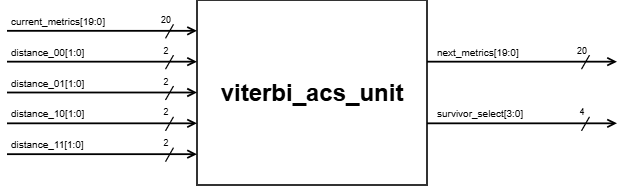
\includegraphics[width=\textwidth,height=6cm,keepaspectratio]{Images/block_diagram/viterbi_acs_unit_block_diagram.png}%
}{%
  \fbox{\parbox[c][6cm][c]{.92\textwidth}{\centering\small
    \code{\detokenize{Images/block_diagram/viterbi_acs_unit_block_diagram.png}}}}%
}
\caption{Block diagram của \code{viterbi\_acs\_unit}}\label{fig:acs-unit-block-diagram}
\end{figure}

Kiến trúc chi tiết bên trong module được trình bày dưới đây.

\begin{figure}[H]\centering
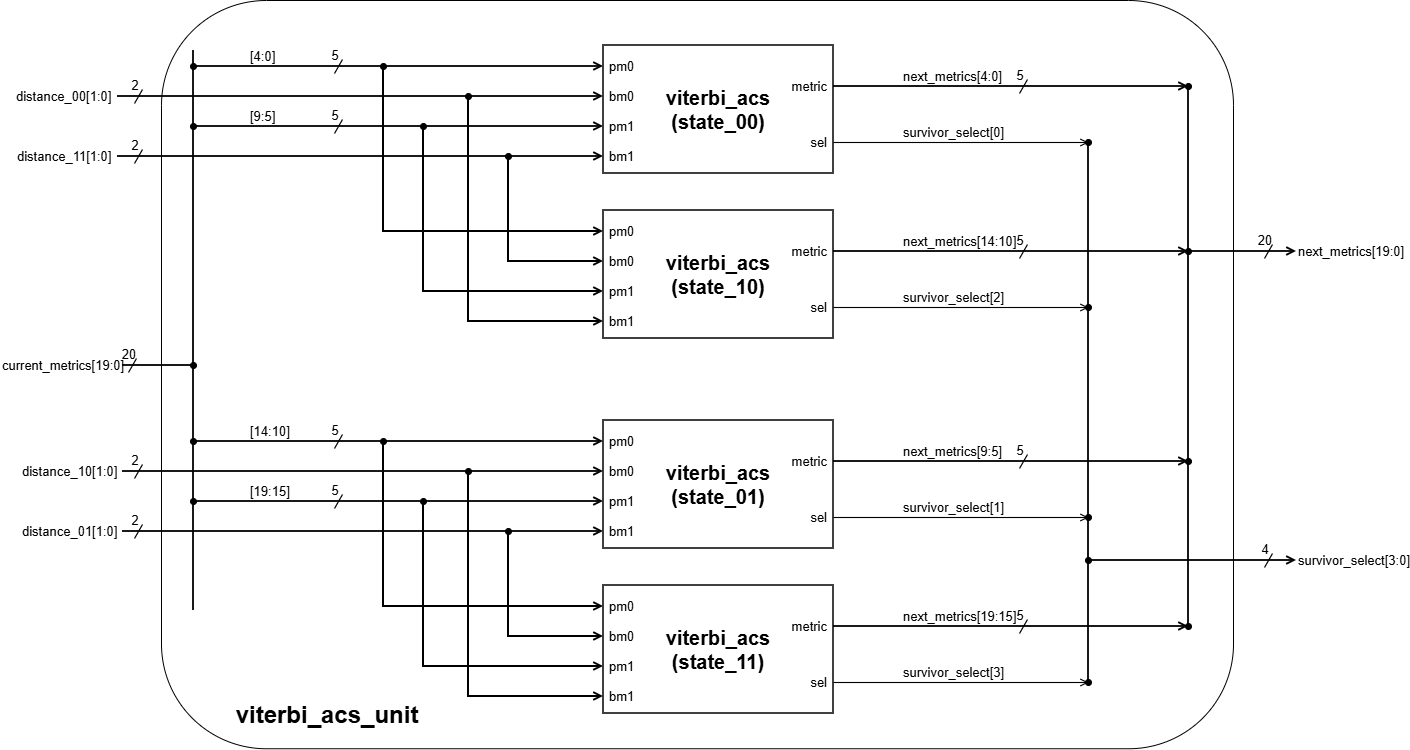
\includegraphics[width=\textwidth,height=.48\textheight,keepaspectratio]{Images/architecture/viterbi_acs_unit_architecture.png}
\caption{Bốn ACS nối song song theo các predecessor của từng trạng thái}\label{fig:acs-unit}
\end{figure}

Bốn instance có tên \code{state\_00}, \code{state\_01}, \code{state\_10} và \code{state\_11}, đều dùng module \code{viterbi\_acs}. Mỗi instance nhận hai metric 5 bit và hai branch metric 2 bit; trả một metric 5 bit và một decision 1 bit. Không có dây điều khiển chọn state khi chạy: các lát bus và các khoảng cách được nối cố định theo trellis.


\subsection{Interface Specification}
\begin{table}[H]\centering\small
\begin{tabularx}{\textwidth}{@{}P{4.0cm}c c Y@{}}\toprule
\textbf{Cổng}&\textbf{Hướng}&\textbf{Số bit}&\textbf{Nội dung}\\\midrule
\code{current\_metrics}&Vào&20&$\{PM11,PM10,PM01,PM00\}$.\\
\code{distance\_00}, \code{distance\_01}&Vào&2 mỗi cổng&Khoảng cách do BMU tính.\\
\code{distance\_10}, \code{distance\_11}&Vào&2 mỗi cổng&Khoảng cách do BMU tính.\\
\code{next\_metrics}&Ra&20&Bốn metric mới, cùng thứ tự với bus vào.\\
\code{survivor\_select}&Ra&4&Bit 0, 1, 2, 3 ứng với state 00, 01, 10, 11.\\
\bottomrule\end{tabularx}
\caption{Giao diện ACS unit và thứ tự các kết quả}\label{tab:acs-unit-ports}
\end{table}



\subsection{Functional Description}
\subsubsection{Các đường đến từng trạng thái}
\begin{table}[H]\centering\small
\begin{tabular}{ccccc}\toprule
\textbf{State đích}&\textbf{Predecessor 0}&\textbf{Predecessor 1}&\textbf{BM đường 0}&\textbf{BM đường 1}\\\midrule
00&00&01&$d_{00}$&$d_{11}$\\01&10&11&$d_{10}$&$d_{01}$\\
10&00&01&$d_{11}$&$d_{00}$\\11&10&11&$d_{01}$&$d_{10}$\\
\bottomrule\end{tabular}
\caption{Ánh xạ predecessor và khoảng cách nhánh trong ACS unit}\label{tab:acs-map}
\end{table}

Chẳng hạn, trạng thái đích 01 chỉ đến từ 10 hoặc 11 với bit vào 0. Hai symbol dự kiến lần lượt là 10 và 01, do đó ACS cho state 01 phải nhận $PM10+d_{10}$ và $PM11+d_{01}$. Đổi nhầm hai branch metric vẫn tạo các con số có vẻ hợp lệ nhưng sẽ giải mã sai trellis.

Ở bước đầu tiên, giả sử symbol nhận là 11. BMU trả $(d_{00},d_{01},d_{10},d_{11})=(2,1,1,0)$. Từ metric đầu $(0,31,31,31)$, bốn ACS trả $(2,31,0,31)$ theo thứ tự trạng thái 00, 01, 10, 11. Kết quả này đúng với trellis: từ state đầu 00 chỉ đi được tới 00 hoặc 10 sau một bit; hai state còn lại vẫn chưa thể tới.


\subsubsection{Hai nhóm predecessor và các lát bus trong ACS unit}
Bốn ACS có thể nhìn thành hai nhóm cùng cặp predecessor. State đích 00 và 10 cùng dùng predecessor 00/01; state đích 01 và 11 cùng dùng predecessor 10/11. Trong mỗi nhóm, hai state đích ứng với bit thông tin khác nhau nên cặp nhãn branch metric được đổi theo trellis.
\begin{table}[H]\centering\small
\begin{tabularx}{\textwidth}{@{}P{2.4cm}P{3cm}P{3cm}Y@{}}\toprule
\textbf{Instance}&\textbf{Metric 0 / metric 1}&\textbf{BM 0 / BM 1}&\textbf{Đích bus}\\\midrule
state\_00&[4:0] / [9:5]&d00 / d11&Next [4:0], decision [0].\\
state\_10&[4:0] / [9:5]&d11 / d00&Next [14:10], decision [2].\\
state\_01&[14:10] / [19:15]&d10 / d01&Next [9:5], decision [1].\\
state\_11&[14:10] / [19:15]&d01 / d10&Next [19:15], decision [3].\\\bottomrule
\end{tabularx}
\caption{Đối chiếu từng cổng instance với bus đóng gói của ACS unit}
\end{table}
Candidate 0 luôn đến từ predecessor có bit nhớ cũ bằng 0. Đây là điều kiện để decision có thể dùng trực tiếp làm bit thấp của predecessor khi truy vết. Nếu đổi thứ tự hai predecessor cho một instance, chỉ giữ nguyên metric min là chưa đủ: ý nghĩa decision của instance đó cũng bị đổi.

Bus next\_metrics phải được ghép theo mã state, không theo thứ tự các instance xuất hiện trong file. Bốn instance có thể viết theo thứ tự bất kỳ trong Verilog, nhưng lát [9:5] vẫn thuộc state 01 và [14:10] vẫn thuộc state 10. Bảng nối cụ thể giúp phân biệt thứ tự văn bản với cấu trúc phần cứng.

Một thử nghiệm cấp khối nên đặt bốn metric vào khác nhau và thay đổi từng distance riêng lẻ. Ví dụ, tăng d00 chỉ tác động ứng viên 0 của state 00 và ứng viên 1 của state 10. Nó không được đi vào hai ACS của nhóm predecessor 10/11. Kiểm tra độ nhạy theo từng đầu vào sẽ phát hiện nhầm dây dễ hơn chỉ dùng tất cả metric bằng nhau.

ACS unit không có thanh ghi và không lưu decision qua chu kỳ. Controller phải lấy cả bus metric mới và vector decision ở cùng cạnh DECODE. Nếu hai bus được chốt ở hai cạnh khác nhau, chúng có thể thuộc hai symbol khác nhau do symbol và metric đầu vào đã thay đổi sau cạnh lấy mẫu.





\subsection{Timing}
Bốn ACS chạy đồng thời và không có thanh ghi giữa đầu vào với đầu ra. Độ trễ khối do đường chậm nhất qua một ACS và các dây nối quyết định, không phải tổng trễ của bốn ACS. Các bus \code{next\_metrics[19:0]} và \code{survivor\_select[3:0]} cần ổn định trước cùng cạnh DECODE. Việc chốt đầu ra ở các cạnh khác nhau sẽ làm metric và decision lệch symbol.
\begin{figure}[H]\centering
% Thay anh trong Images de cap nhat so do; khong ve bang TikZ.
\IfFileExists{Images/waveform/waveform_viterbi_acs_unit.png}{%
  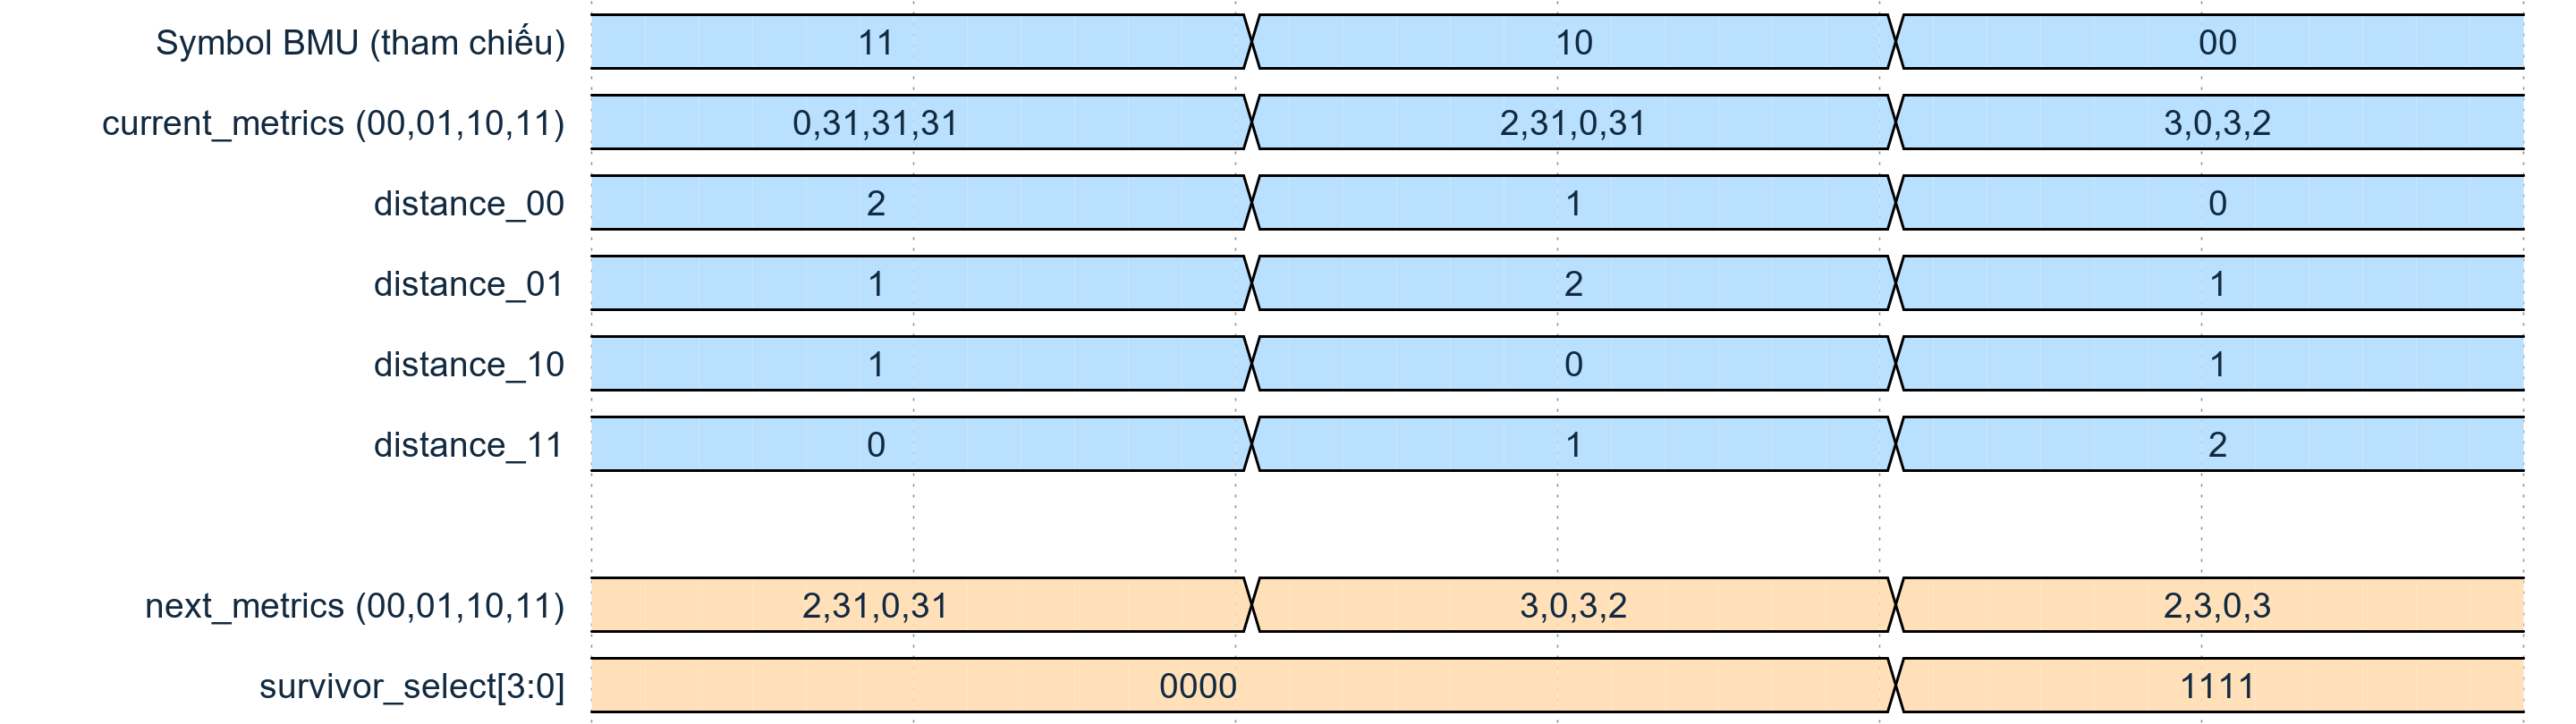
\includegraphics[width=\linewidth,height=4cm,keepaspectratio]{Images/waveform/waveform_viterbi_acs_unit.png}%
}{%
  \fbox{\parbox[c][4cm][c]{.92\linewidth}{\centering\small
    \code{\detokenize{Images/waveform/waveform_viterbi_acs_unit.png}}}}%
}
\caption{Bốn metric mới và bốn decision ứng với cùng một bộ đầu vào}\label{fig:acs-unit-waveform}
\end{figure}

Trong Hình~\ref{fig:acs-unit-waveform}, mỗi khoảng ứng với một symbol nhận được. Bốn giá trị trên mỗi bus metric được đọc từ trái sang phải theo thứ tự trạng thái $(00,01,10,11)$. Với symbol đầu tiên \texttt{11}, chỉ trạng thái trước \texttt{00} có metric hữu hạn. Hai nhánh từ trạng thái này đến đích \texttt{00} và \texttt{10} có khoảng cách lần lượt là~2 và~0. Do đó, bộ metric ban đầu $(0,31,31,31)$ cho kết quả $(2,31,0,31)$. Bộ điều khiển dùng kết quả này làm \texttt{current\_metrics} cho symbol thứ hai \texttt{10}, sau đó thu được $(3,0,3,2)$.

Ở khoảng thứ ba, symbol \texttt{00} cho $d_{00}=0$ và $d_{11}=2$. Xét riêng trạng thái đích \texttt{00}, đường từ trạng thái trước \texttt{00} có metric $3+0=3$, còn đường từ \texttt{01} có metric $0+2=2$. ACS giữ đường thứ hai. Vì vậy, phần tử đầu của \texttt{next\_metrics} giảm từ~3 xuống~2 và bit~0 của \texttt{survivor\_select} chuyển từ~0 lên~1. Ba ACS còn lại cũng chọn đường~1, nên vector quyết định cho bước này là \texttt{1111}.



\subsection{Verification Requirements}
% TODO: Bo sung yeu cau kiem chung o buoc tiep theo.

\clearpage\section{ĐẶC TẢ MODULE \code{viterbi\_best\_state}}\label{sec:best-state}
\subsection{Overview \& Scope}
\code{viterbi\_best\_state} đọc bốn metric cuối, so sánh cặp 00/01 và cặp 10/11, sau đó so sánh hai giá trị thắng. Cấu trúc cây có hai tầng so sánh theo đường dữ liệu, thay cho ba phép so sánh nối tiếp.


\subsection{Architecture}
Hình~\ref{fig:best-state-block-diagram} là block diagram của \code{viterbi\_best\_state}, thể hiện tên, hướng và độ rộng các cổng vào/ra.

\begin{figure}[H]\centering
% Tai anh block diagram tong cua module len Images voi dung ten file nay.
\IfFileExists{Images/block_diagram/viterbi_best_state_block_diagram.png}{%
  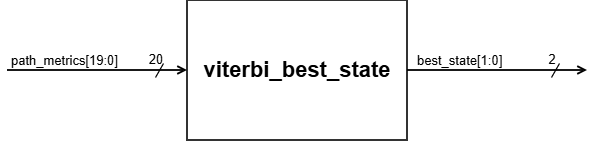
\includegraphics[width=\textwidth,height=6cm,keepaspectratio]{Images/block_diagram/viterbi_best_state_block_diagram.png}%
}{%
  \fbox{\parbox[c][6cm][c]{.92\textwidth}{\centering\small
    \code{\detokenize{Images/block_diagram/viterbi_best_state_block_diagram.png}}}}%
}
\caption{Block diagram của \code{viterbi\_best\_state}}\label{fig:best-state-block-diagram}
\end{figure}

Kiến trúc chi tiết bên trong module được trình bày dưới đây.

\begin{figure}[H]\centering
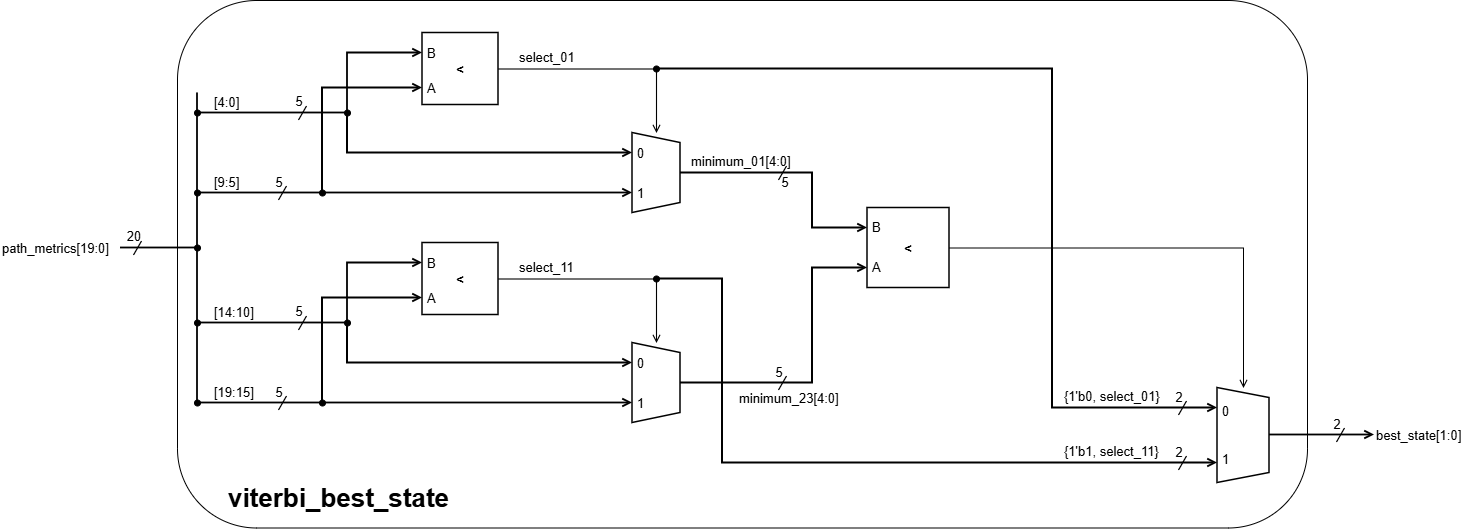
\includegraphics[width=\textwidth,height=.43\textheight,keepaspectratio]{Images/architecture/viterbi_best_state_architecture.png}
\caption{Cây so sánh chọn trạng thái có path metric nhỏ nhất}\label{fig:best-state}
\end{figure}

Tầng đầu so hai cặp metric độc lập. Tầng sau so hai metric nhỏ nhất và ghép mã trạng thái 2 bit.
\begin{table}[H]\centering\small
\begin{tabularx}{\textwidth}{@{}P{3.6cm}c Y@{}}\toprule
\textbf{Dây}&\textbf{Số bit}&\textbf{Hướng truyền dữ liệu}\\\midrule
\code{select\_01}&1&So sánh PM01/PM00 $\rightarrow$ MUX \code{minimum\_01} và bit mã trạng thái.\\
\code{select\_11}&1&So sánh PM11/PM10 $\rightarrow$ MUX \code{minimum\_23} và bit mã trạng thái.\\
\code{minimum\_01}&5&MUX cặp 00/01 $\rightarrow$ comparator tầng cuối.\\
\code{minimum\_23}&5&MUX cặp 10/11 $\rightarrow$ comparator tầng cuối.\\
\code{best\_state}&2&Chọn nhóm và mã trong nhóm $\rightarrow$ cổng ra.\\
\bottomrule\end{tabularx}
\caption{Tên và độ rộng các dây trong bộ chọn trạng thái cuối}\label{tab:best-wires}
\end{table}


\subsection{Interface Specification}
\begin{table}[H]\centering\small
\begin{tabularx}{\textwidth}{@{}P{4cm}c c Y@{}}\toprule
\textbf{Cổng}&\textbf{Hướng}&\textbf{Số bit}&\textbf{Ý nghĩa}\\\midrule
\code{path\_metrics}&Vào&20&Metric theo thứ tự $\{PM11,PM10,PM01,PM00\}$.\\
\code{best\_state}&Ra&2&Mã state có metric nhỏ nhất.\\
\bottomrule\end{tabularx}
\caption{Giao diện bộ chọn trạng thái cuối}\label{tab:best-ports}
\end{table}



\subsection{Functional Description}

\begin{table}[H]\centering\small
\begin{tabular}{ccccc}\toprule
\textbf{PM00}&\textbf{PM01}&\textbf{PM10}&\textbf{PM11}&\textbf{Best state}\\\midrule
0&3&4&5&00\\4&1&2&3&01\\9&8&2&4&10\\9&8&7&3&11\\
5&5&5&5&00\\8&2&2&7&01\\
\bottomrule\end{tabular}
\caption{Ví dụ chọn state cuối, gồm trường hợp hòa giữa hai nhánh cây}\label{tab:best-examples}
\end{table}
Mọi phép chọn đều chỉ đổi sang state có chỉ số lớn hơn khi metric của nó \emph{nhỏ hơn} nghiêm ngặt. Vì thế, nếu nhiều trạng thái cùng đạt metric nhỏ nhất, đầu ra là chỉ số nhỏ nhất. Không được thay quy tắc này bằng chọn tùy ý nếu muốn kết quả bit khớp mô hình tham chiếu trong các trường hợp hòa.

Khối luôn tính theo bus metric hiện tại, kể cả khi khung chưa kết thúc. Chỉ giá trị được controller chốt trong SELECT\_FINAL\_STATE mới là state cuối của khung. Vì không có tail bit bắt buộc, không thể bỏ khối này và mặc định bắt đầu traceback từ 00.


\subsubsection{Phân tích chi tiết cây so sánh của best-state}
Bộ chọn state cuối cần trả cả metric thắng nội bộ và mã state gắn với metric đó. Tầng đầu so PM01 với PM00, và PM11 với PM10. Mỗi nhánh tạo một giá trị nhỏ nhất cùng một bit chỉ ra state nào trong cặp được giữ. Tầng cuối chọn giữa hai cặp.
\begin{equation}
\begin{aligned}
s_{01}&=(PM01<PM00),&m_{01}&=s_{01}?PM01:PM00,\\
s_{23}&=(PM11<PM10),&m_{23}&=s_{23}?PM11:PM10.
\end{aligned}
\end{equation}
Nếu $m_{23}<m_{01}$, state thắng là $\{1,s_{23}\}$; ngược lại là $\{0,s_{01}\}$. Bit cao đánh số nhóm, bit thấp đánh số state trong nhóm. Cổng ngoài chỉ trả mã state, không xuất metric nhỏ nhất hay cờ độ tin cậy.

\begin{table}[H]\centering\small
\begin{tabular}{cccccc}\toprule
\textbf{PM00}&\textbf{PM01}&\textbf{PM10}&\textbf{PM11}&\textbf{Hai min}&\textbf{State}\\\midrule
7&2&2&8&2 / 2&01\\4&4&1&1&4 / 1&10\\3&3&3&3&3 / 3&00\\31&31&31&31&31 / 31&00\\\bottomrule
\end{tabular}
\caption{Xử lý hòa tại một cặp và giữa hai cặp metric}
\end{table}
Khi hòa trong cặp, phép so sánh nghiêm ngặt giữ state nhỏ hơn. Khi hòa giữa hai cặp, chọn nhóm có bit cao 0. Kết hợp hai quy tắc bảo đảm state cuối nhỏ nhất trong tập các state có metric tối thiểu, kể cả khi có ba hoặc bốn state cùng thắng.

Trường hợp cả bốn metric bằng 31 cho đầu ra 00 là kết quả logic của cây, không phải chứng nhận có đường hữu hạn. Trong vận hành hợp lệ của khung bắt đầu ở 00, luôn có ít nhất một đường hữu hạn, nên trường hợp toàn vô cực không được dùng làm một tín hiệu phát hiện lỗi hệ thống.

Độ sâu hai tầng so sánh là mô tả cấu trúc, không tự xác định độ trễ ns. Các MUX chọn giá trị ở tầng đầu và dây nối đến comparator cuối cũng nằm trên đường timing. Controller đã dành một chu kỳ sau lần cập nhật metric cuối trước khi chốt best\_state; chức năng đúng không thay thế được kiểm tra setup/hold của đường này.



\begin{table}[H]\centering\small
\begin{tabularx}{\textwidth}{@{}P{5.6cm}P{3.5cm}Y@{}}\toprule
\textbf{Điều kiện}&\textbf{Nếu đúng}&\textbf{Nếu sai, kể cả bằng nhau}\\\midrule
$PM01<PM00$&\code{select\_01=1}&Chọn PM00 nếu không nhỏ hơn.\\
$PM11<PM10$&\code{select\_11=1}&Chọn PM10 nếu không nhỏ hơn.\\
$minimum_{23}<minimum_{01}$&\code{best\_state}=$\{1,select_{11}\}$&Chọn nhóm 00/01 nếu không nhỏ hơn.\\
\bottomrule\end{tabularx}
\caption{Các phép so sánh và quy tắc giữ trạng thái nhỏ hơn}\label{tab:best-selection}
\end{table}


\subsection{Timing}
Đầu ra là tổ hợp, không đợi clock. Sau cạnh cập nhật metric thứ tám $N+8$, cây so sánh tính theo bốn metric mới. Controller chốt \code{best\_state} tại $N+9$, do đó đường từ thanh ghi metric qua hai tầng comparator/MUX đến thanh ghi truy vết có một chu kỳ để ổn định. Không dùng kết quả lấy trước $N+8$ làm trạng thái cuối của khung.
\begin{figure}[H]\centering
% Thay anh trong Images de cap nhat so do; khong ve bang TikZ.
\IfFileExists{Images/waveform/waveform_viterbi_best_state.png}{%
  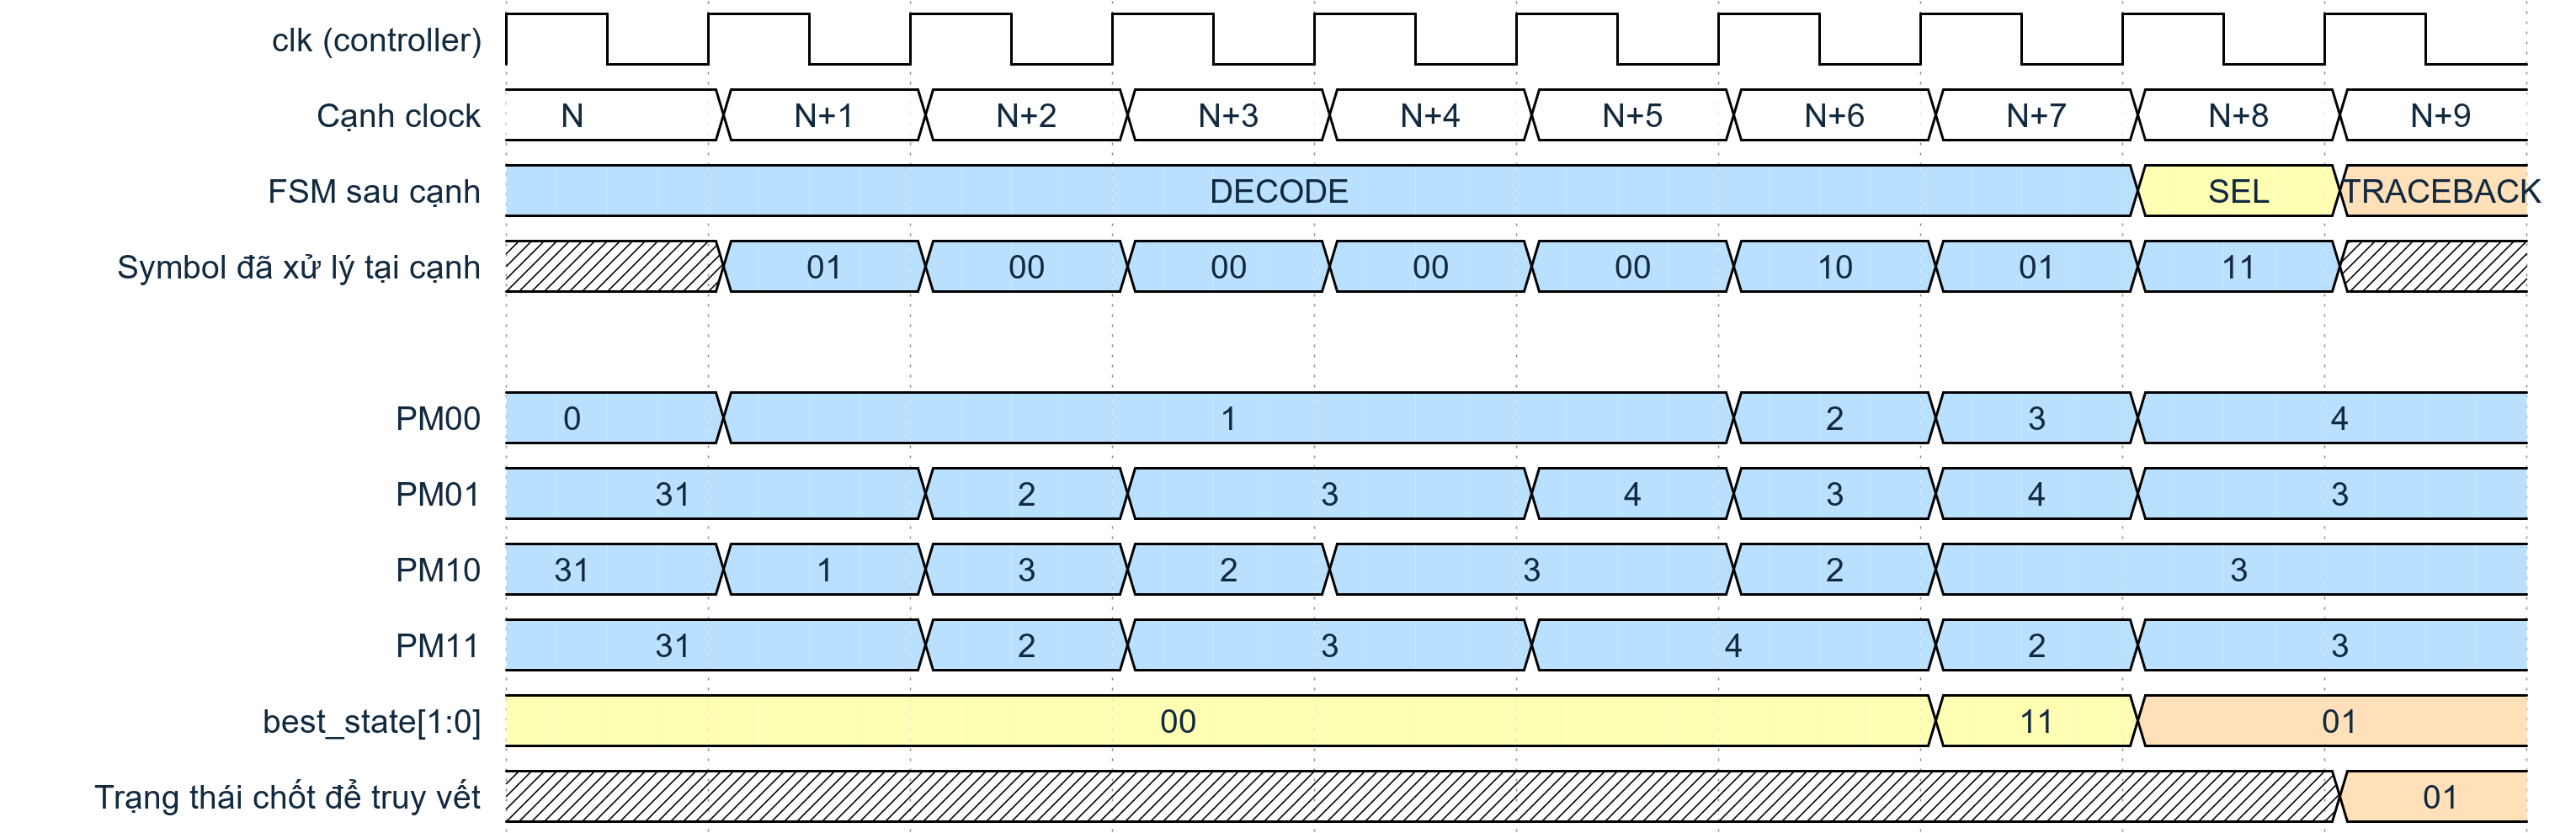
\includegraphics[width=\linewidth,height=4cm,keepaspectratio]{Images/waveform/waveform_viterbi_best_state.png}%
}{%
  \fbox{\parbox[c][4cm][c]{.92\linewidth}{\centering\small
    \code{\detokenize{Images/waveform/waveform_viterbi_best_state.png}}}}%
}
\caption{Metric cuối sau $N+8$ và thời điểm chốt trạng thái truy vết tại $N+9$}\label{fig:best-waveform}
\end{figure}
Hình~\ref{fig:best-waveform} theo dõi khung \texttt{0x4027} từ cạnh nhận khung $N$ đến cạnh bắt đầu truy vết $N+9$. Tại $N$, bộ metric $(PM_{00},PM_{01},PM_{10},PM_{11})$ được khởi tạo bằng $(0,31,31,31)$. Từ $N+1$ đến $N+8$, hàng symbol cho biết cặp bit vừa được xử lý tại mỗi cạnh. Bốn hàng metric bên dưới là kết quả sau khi bộ điều khiển đã chốt cập nhật của cặp bit đó.

Tại $N+7$, bộ metric là $(3,4,3,2)$. Trạng thái \texttt{11} có metric nhỏ nhất nên \texttt{best\_state} bằng \texttt{11}. Sau cạnh $N+8$, symbol cuối \texttt{11} đưa bộ metric về $(4,3,3,3)$. Ba trạng thái \texttt{01}, \texttt{10} và \texttt{11} cùng đạt metric~3. Theo quy tắc ưu tiên mã trạng thái nhỏ nhất khi hòa, đầu ra tổ hợp \texttt{best\_state} chuyển sang \texttt{01}. Giá trị này ổn định trong pha chọn trạng thái cuối và được bộ điều khiển chốt tại cạnh $N+9$, như thể hiện ở hàng cuối của hình.



\subsection{Verification Requirements}
% TODO: Bo sung yeu cau kiem chung o buoc tiep theo.

\clearpage
\section{KIỂM CHỨNG VÀ CÁC RÀNG BUỘC THIẾT KẾ}
\subsection{Phương pháp kiểm chứng chức năng}
Mô hình tham chiếu trong \code{scripts/run\_tests.py} tạo đủ 256 từ mã từ 256 byte thông tin, rồi tìm khoảng cách Hamming nhỏ nhất đối với từng từ nhận 16 bit. Cách kiểm tra này không dùng lại mạng trellis hoặc ACS của DUT, nên có thể phát hiện sai ánh xạ nhánh cũng như sai thuật toán cập nhật metric.

Ngoài giá trị đầu ra, testbench cần kiểm tra giao thức: chỉ nhận khung khi IDLE, không lấy lại bus ngoài sau khi chốt, hoàn tất đúng cạnh $N+17$, \code{done} dài một chu kỳ và đầu ra giữ ổn định giữa hai lần hoàn tất. Reset được kích ở nhiều pha để kiểm tra hủy khung và phục hồi. Các trường hợp hòa phải so với quy tắc đã công bố, thay vì chấp nhận tùy ý một byte có cùng khoảng cách.

\subsection{Ma trận yêu cầu cần kiểm tra}
\small
\begin{longtable}{@{}P{1.7cm}P{7.4cm}P{5.9cm}@{}}
\caption{Yêu cầu kiểm chứng và cách quan sát}\label{tab:verification}\\
\toprule\textbf{ID}&\textbf{Điều cần xác nhận}&\textbf{Phương pháp}\\\midrule\endfirsthead
\toprule\textbf{ID}&\textbf{Điều cần xác nhận}&\textbf{Phương pháp}\\\midrule\endhead
SYS-01&Khung 16 bit cho kết quả đúng theo khoảng cách Hamming nhỏ nhất.&So với codebook độc lập cho toàn bộ 65.536 từ nhận.\\
SYS-02&Cả hai chế độ đóng gói bit hoạt động đúng.&Dùng hai DUT, vector không đối xứng và kiểm tra vị trí từng bit.\\
SYS-03&Nhận khung ở cạnh $N$, trả kết quả ở $N+17$, nhận lại sớm nhất $N+18$.&Đếm cạnh; kiểm tra busy/done và start giữ cao.\\
SYS-04&Start lúc busy không ghi đè khung; đổi bus ngoài không ảnh hưởng khung đã nhận.&Đổi start và encoded\_data trong DECODE/TRACEBACK.\\
CTL-01&Metric đầu là $(0,31,31,31)$ ở mỗi khung.&Quan sát ngay sau reset và cạnh nhận start.\\
CTL-02&Ghi đủ hàng survivor 0--7 trước TRACEBACK.&Kiểm tra địa chỉ ghi, số lần ghi và chuyển pha ở chỉ số 7.\\
CTL-03&State cuối dùng metric của đủ tám symbol.&Đối chiếu metric sau $N+8$ với state chốt ở $N+9$.\\
CTL-04&Không thiếu bit cuối khi chốt đầu ra.&Chọn vector có $u_0=1$; so decoded\_next và decoded\_data ở bước cuối.\\
CTL-05&Reset hủy khung, xóa done/đầu ra; khung sau vẫn đúng.&Reset ở DECODE, SELECT\_FINAL\_STATE và TRACEBACK.\\
BM-01&Bốn khoảng cách đúng và nằm trong 0--2.&Kiểm tra vét cạn bốn symbol theo Bảng~\ref{tab:bmu-truth}.\\
ACS-01&Cộng mở rộng, bão hòa ở 31, không tràn về 0.&Vector quanh ngưỡng và predecessor bằng 31.\\
ACS-02&Hòa chọn candidate 0; metric khớp decision.&Vector nhỏ hơn, lớn hơn và bằng nhau.\\
AU-01&Bốn instance nhận đúng predecessor và branch metric.&So từng hàng Bảng~\ref{tab:acs-map} với mô hình tổ hợp.\\
AU-02&Metric và decision đúng lát bus/state.&Đặt metric phân biệt, kiểm tra cả bốn đầu ra.\\
BS-01&Chọn metric nhỏ nhất; hòa chọn state nhỏ nhất.&Đổi vị trí cực tiểu; kiểm tra hòa trong và giữa hai cặp.\\
TB-01&Đọc đúng hàng và decision; ghép đủ tám bit.&So state/bit từng bước với truy vết tham chiếu.\\
TB-02&Thứ tự ghi MSB-first là [0] đến [7] khi truy vết ngược.&Đối chiếu Mục~\ref{sec:control-traceback}.\\
PHY-01&Đạt clock, diện tích, công suất trong công nghệ được giao.&Synthesis, STA và power analysis với ràng buộc đầy đủ.\\
\bottomrule\end{longtable}
\normalsize


\subsection{Kế hoạch kiểm tra riêng từng phần tử tổ hợp}
Kiểm tra cấp cell giúp định vị lỗi trước khi chạy khung hoàn chỉnh. Các miền đầu vào dưới đây đủ nhỏ để vét cạn khi cần. Chúng là phạm vi kiểm thử đề xuất cho lần phát triển tiếp theo; báo cáo không xem chúng là các lượt chạy mới đã có log.
\begin{table}[H]\centering\small
\begin{tabularx}{\textwidth}{@{}P{3.2cm}P{3.2cm}Y@{}}\toprule
\textbf{Khối}&\textbf{Số tổ hợp}&\textbf{Nội dung so sánh}\\\midrule
BMU&4&Đủ bốn đầu ra và miền 0--2.\\
ACS, BM hợp lệ&$32^2\times3^2=9216$&Tổng mở rộng, bão hòa, select và metric.\\
ACS, đủ mã bus BM&$32^2\times4^2=16384$&Thêm mã BM=3 để thử giao diện cell.\\
Best-state&$32^4=1048576$&Giá trị argmin và chọn state nhỏ nhất khi hòa.\\
ACS unit&Vector định hướng và ngẫu nhiên có seed&Đúng ánh xạ từng predecessor, nhãn và lát bus.\\\bottomrule
\end{tabularx}
\caption{Không gian kiểm thử cấp khối và mục đích của từng phép thử}
\end{table}
Mô hình ACS nên tính tổng bằng kiểu số nguyên rộng, áp dụng min với 31 rồi so sánh; không nên dùng lại cùng cách cắt bit của DUT. Mô hình best-state có thể duyệt bốn state theo thứ tự tăng dần và chỉ thay kết quả khi tìm được metric nhỏ hơn. Hai cách này đơn giản nhưng có cấu trúc khác mạng cổng đang được kiểm tra.

Với controller, phép kiểm tra cần quan sát sự kiện, không chỉ giá trị cuối. Tám lần ghi survivor phải xuất hiện ở các địa chỉ 0--7; sau đó không còn ghi trong pha ngược. Done không được lên trước lần đọc địa chỉ 0, và một start lúc busy không được thay encoded\_shift bằng bus ngoài.

\begin{table}[H]\centering\small
\begin{tabularx}{\textwidth}{@{}P{4cm}Y@{}}\toprule
\textbf{Vector nhắm lỗi}&\textbf{Lỗi có thể phát hiện}\\\midrule
Bit đầu theo thời gian bằng 1&Thiếu bit cuối của traceback khi chốt từ bộ đệm cũ.\\
Tất cả metric khác nhau&Đảo state, đảo lát bus hoặc sai comparator.\\
Hai candidate bằng nhau&Đổi quy tắc tie-break ngoài ý muốn.\\
Reset giữa pha tiến rồi nhận lại&Đọc survivor cũ trước khi ghi đủ khung mới.\\
Start giữ cao qua done&Sai khoảng cách nhận hai khung 18 chu kỳ.\\\bottomrule
\end{tabularx}
\end{table}
Đạt kiểm tra chức năng không làm hoàn tất kiểm tra vật lý. Không có delay trong RTL nên testbench không thể tự xác nhận tần số tối đa, công suất hay diện tích của thư viện cell. Các bước STA và power analysis vẫn là các bằng chứng riêng cần có theo flow thực tế.


\subsection{Kết quả mô phỏng đã được lưu trong dự án}
Thư mục \code{verification/} có log regression và tệp tổng hợp kết quả; tài liệu \code{VERIFICATION.md} ghi lần kiểm tra ngày 28/10/2026. Các số liệu trong Bảng~\ref{tab:existing-results} được trích từ các tệp này, không phải một lượt chạy RTL mới khi biên soạn báo cáo.
\begin{table}[H]\centering\small
\begin{tabularx}{\textwidth}{@{}P{4.4cm}Y@{}}\toprule
\textbf{Hạng mục}&\textbf{Kết quả đã ghi nhận}\\\midrule
Không gian từ nhận&65.536 từ 16 bit; kiểm tra ở cả LSB-first và MSB-first.\\
Khung sạch&Đủ 256 byte thông tin được kiểm tra.\\
Reset và phục hồi&Năm trường hợp phục hồi sau khi hủy khung.\\
Log testbench decoder&\code{PASS: 65797 frames in BOTH bit-order modes; all 65536 received words}.\\
Giao tiếp bằng file&\code{PASS: 256 file vectors}; dữ liệu mẫu được sinh để thử.\\
Dữ liệu chính thức của giảng viên&Chưa được kiểm tra theo tệp tổng hợp hiện có.\\
PPA vật lý&Chưa được xác nhận.\\
\bottomrule\end{tabularx}
\caption{Kết quả chức năng có sẵn trong hồ sơ kiểm chứng}\label{tab:existing-results}
\end{table}
Các kết quả trên xác nhận phạm vi đã chạy theo log, không thay cho mọi phép kiểm tra cấp cell trong ma trận. Kiểm tra vét cạn từ nhận cũng không có nghĩa mạch sửa đúng mọi mẫu lỗi: điều được kiểm tra là nghiệm có khoảng cách nhỏ nhất và quy tắc phân xử hòa, kể cả khi nghiệm đó khác bản tin thực sự đã truyền.

\subsection{Mục tiêu PPA và các đường cần phân tích timing}
\begin{table}[H]\centering\small
\begin{tabularx}{\textwidth}{@{}P{3.2cm}P{3.5cm}Y@{}}\toprule
\textbf{Chỉ tiêu}&\textbf{Mục tiêu}&\textbf{Bằng chứng cần có}\\\midrule
Tần số&$f_{clk}\ge200\ \mathrm{MHz}$&STA với clock 5 ns và đầy đủ ràng buộc IO, uncertainty.\\
Diện tích&$\le7000\ \mu\mathrm{m}^2$&Báo cáo ánh xạ cell theo thư viện và flow được giao.\\
Công suất&$\le1.5\ \mathrm{mW}$&Power analysis với điện áp, corner và hoạt động chuyển mạch xác định.\\
\bottomrule\end{tabularx}
\caption{Mục tiêu PPA cấp toàn thiết kế}\label{tab:ppa}
\end{table}
Vòng cập nhật metric gồm đường từ \code{path\_metrics} qua phép cộng, bão hòa, so sánh và MUX của ACS rồi quay về thanh ghi metric. Một nhánh đầu vào khác đi từ \code{encoded\_shift} qua BMU đến ACS. Cả hai cần được kiểm tra; chưa có báo cáo STA để kết luận nhánh nào là critical path thực tế.

Pha chọn state có đường từ thanh ghi metric qua cây so sánh hai tầng đến \code{traceback\_state}. Pha traceback có đường từ chỉ số và state qua mạng chọn hàng/bit survivor, rồi quay về state hoặc tới logic ghi bit. Dù bộ nhớ chỉ có 32 bit, các MUX chọn động vẫn đóng góp độ trễ. Thời gian thiết lập, clock-to-Q, skew và tải dây phải được tính trong ngân sách 5 ns.

Tệp \code{constraints/viterbi\_decoder.sdc} đặt clock mục tiêu 5 ns. Khi chạy flow vật lý cần bổ sung điều kiện IO, tải, driving cell, uncertainty và xử lý reset phù hợp. Clock 5 ns trong mô phỏng chỉ kiểm tra lịch giao thức; các chỉ tiêu tần số, diện tích và công suất chỉ được kết luận sau khi có báo cáo tương ứng.

\clearpage
\section{KẾT LUẬN}
Bộ giải mã sử dụng bốn ACS song song để xử lý trellis bốn trạng thái, lưu 32 bit quyết định survivor và truy vết đủ tám bước cho mỗi khung. Controller bảo đảm các kết quả metric được lưu cùng decision, state cuối được chọn sau lần cập nhật thứ tám và byte đầu ra chỉ thay đổi khi đã ghép đủ tám bit.

Giao diện có thời gian xử lý cố định: nhận khung ở IDLE, trả kết quả sau 17 chu kỳ và có thể nhận khung tiếp theo sau 18 chu kỳ. Hai chế độ đóng gói dữ liệu dùng chung thuật toán và FSM; sự khác biệt nằm ở đầu lấy symbol và vị trí ghi bit trong bộ đệm. Đây là các quy ước cần giữ thống nhất giữa encoder, decoder và testbench khi tích hợp.

Hồ sơ dự án đã có kết quả kiểm chứng chức năng trên toàn bộ không gian từ nhận 16 bit ở hai chế độ. Công việc còn lại ở mức triển khai là xác nhận timing, diện tích và công suất với thư viện công nghệ và điều kiện hoạt động cụ thể.

\begin{thebibliography}{99}
\raggedright
\addcontentsline{toc}{section}{\refname}
\bibitem{mit-lecture} MIT 6.02, \emph{Lecture 9: Viterbi Decoding of Convolutional Codes}, 2010.

\bibitem{oshea-thesis} John O'Shea, \emph{Efficient ASIC Design of Viterbi Decoders}, luận văn Master of Engineering, University of Limerick, 2001.

\bibitem{odroma-storage} M. O'Droma và J. O'Shea, \emph{FPGA Based Storage Efficient Viterbi Decoders}, University of Limerick.

\bibitem{tervo-viterbi} Richard Tervo, University of New Brunswick, ECE4253, \href{https://www.ece.unb.ca/tervo/ece4253/convolution1.shtml}{\emph{Convolutional Coding}}, \href{https://www.ece.unb.ca/tervo/ece4253/convolution2.shtml}{\emph{Convolutional Coding -- Decoding}} và \href{https://www.ece.unb.ca/tervo/ece4253/convolution3.shtml}{\emph{Convolutional Coding -- Viterbi Decoding}}.

\end{thebibliography}

\end{document}